\documentclass[10pt,b5paper,twoside,openright]{book}
\usepackage{config}

% From https://www.overleaf.com/learn/latex/Glossaries

\makeglossaries % Prepare for adding glossary entries


\newglossaryentry{BnB}
{
        name=B\&B,
        description={Branch and Bound}
}

\newglossaryentry{DP}
{
        name=DP,
        description={Dynamic Programming}
}

\newglossaryentry{MILP}
{
        name=MILP,
        description={Mixed Integer Linear Programming}
}

\newglossaryentry{MIP}
{
        name=MIP,
        description={Mixed Integer Programming}
}

\newglossaryentry{MINLP}
{
        name=MINLP,
        description={Mixed Integer Non-Linear Programming}
}
 
\newglossaryentry{SCIP}
{
        name=SCIP,
        description={Solving Constraint Integer Programs}
}

\newglossaryentry{MLP}
{
        name=MLP,
        description={Multi-Layer Perceptron}
}

\newglossaryentry{ML}
{
        name=ML,
        description={Machine Learning}
}

\newglossaryentry{AI}
{
        name=AI,
        description={Artificial Intelligence}
}

\newglossaryentry{LP}
{
        name=LP,
        description={Linear Programming}
}

\newglossaryentry{ILP}
{
        name=ILP,
        description={Integer Linear Programming}
}

\newglossaryentry{BLP}
{
        name=BLP,
        description={Binary Linear Programming}
}

\newglossaryentry{SB}
{
        name=SB,
        description={Strong Branching}
}

\newglossaryentry{GCNN}
{
        name=GCNN,
        description={Graph Convolutional Neural Networks}
}

\newglossaryentry{GNN}
{
        name=GCNN,
        description={Graph (Convolutional) Neural Networks}
}

\newglossaryentry{ReLU}
{
        name=ReLU,
        description={Recti-Linear Unit}
}

\newglossaryentry{FSB}
{
        name=FSB,
        description={Full Strong Branching}
}

\newglossaryentry{MIB}
{
        name=MIB,
        description={Most Infeasible Branching}
}

\newglossaryentry{PC}
{
        name=PB,
        description={Pseudo-cost Branching}
}

\newglossaryentry{RPC}
{
        name=RPB,
        description={Reliability Pseudo-cost Branching}
}

\newglossaryentry{NP}
{
        name=NP,
        description={Non-deterministic Polynomial-time}
}

\newglossaryentry{CPU}
{
        name=CPU,
        description={Central Processing Unit}
}

\newglossaryentry{GPU}
{
        name=GPU,
        description={Graphics Processing Unit}
}

\newglossaryentry{FiLM}
{
        name=FiLM,
        description={Feature-wise Linear Modulation}
}

\newglossaryentry{SVM}
{
        name=SVM,
        description={Support Vector Machine}
}

\newglossaryentry{COIN-OR}
{
        name=COIN-OR,
        description={Computational Infrastructure for Operations Research}
}

\newglossaryentry{MDP}
{
        name=MDP,
        description={Markov Decision Process}
}

\newglossaryentry{PO-MDP}
{
        name=PO-MDP,
        description={Partially-observable Markov Decision Process}
}

\newglossaryentry{CO}
{
        name=CO,
        description={Combinatorial Optimization}
}

\newglossaryentry{RL}
{
        name=RL,
        description={Reinforcement Learning}
}

\newglossaryentry{DS4DM}
{
        name=DS4DM,
        description={Canada Excellence Research Chair in Data Science for Decision Making}
}

\newglossaryentry{Ecole}
{
        name=Ecole,
        description={Extensible Combinatorial Optimization Learning Environments}
}

\newglossaryentry{IA}
{
        name=IA,
        description={Iterative Ablations}
}

\addbibresource{bib/bibliography.bib}
\setlength{\cftbeforesecskip}{5pt}
\begin{document}

\pagestyle{empty}
\newcommand{\HRule}{\rule{\linewidth}{1mm}}
 
\vspace*{\stretch{1}}
\vspace*{-3.5cm}
\noindent\HRule
\begin{center}
 
\end{center}
\begin{center}
  \huge
	\large
	\noindent\emph{Engineering Cybernetics\\TTK4550 Specialization Project}
\end{center}
\begin{center}
 
\end{center}
\begin{center}
	\huge
	\noindent\emph{}
  \huge
  \Large
  \noindent \textbf{Multi-Layer Perceptrons for Branching in Mixed-Integer Linear Programming}
  \\ [7mm]
  \large
  \noindent\emph{Lars Lødemel Sandberg}
\end{center}
\begin{center}
  \huge
  \large
  \noindent\emph{Supervisors:\\ Prof. Lars Struen Imsland \\ Arild Helseth}
\end{center}
\begin{center}
	\large
	\noindent \emph{Trondheim, 17 December 2020}
	%\noindent \emph{Trondheim, 15 June 2007}
\end{center}
\noindent\HRule
\vspace*{\stretch{2}}
\begin{figure}[h]
	\begin{center}
		
\includegraphics[angle=0, width=10cm]{img/logo_ntnu}
	\end{center}
	\label{fig:logo}
\end{figure}
 
\begin{minipage}[c]{\textwidth}
	{\setlength{\baselineskip}{0.5\baselineskip}
	\small \noindent Faculty of Information Technology and Electrical Engineering\\
	\Large \noindent \textsc{department of engineering cybernetics}}
\end{minipage}

\frontmatter
\pagestyle{plain}

\begingroup
\let\cleardoublepage\clearpage
%!TEX root = ../thesis.tex
\chapter*{\englishabstractname}
\addcontentsline{toc}{chapter}{\englishabstractname}
% Multilayer Perceptrons for Learning to Branch
%
This project evaluates Multi-layer Perceptrons for machine learning aided branching proposed by Gupta et al. \cite{gupta2020hybrid}
for faster solving Mixed-Integer Linear Programming (\gls{MILP}) problems. 
Efficient \gls{MILP} solution algorithms are important for real-time optimization in various industries, including industrial production, logistics, transportation, and energy production \cite{junger2010years}.  % Reduced computation time via merging Machine learning with the Branch and Bound solution algorithm can improve these algorithms without sacrificing the strong benefits global optimization has over purely data-driven methods.
Multiple central researchers within mathematical programming and machine learning have recently shown interest in the application of Machine Learning in \gls{MILP} \cite{bengio2020machine,bertsimas2019online}. Particularly the variable selection part of the branching strategy has proved to be a field where machine learning methods can give promising results \cite{khalil2020towards}.
In 2019, reliable results of improvement over top branching strategies in open-source solvers were shown \cite{gasse2019exact}, and in 2020 these methods have been expanded to purely \gls{CPU}-based solutions \cite{gupta2020hybrid}. Multi-Layer Perceptrons are included in Gupta et al. \cite{gupta2020hybrid}, however their efficiency is not reported, and neither is it clear whether their configuration is significant to the resulting solution time.

In order to address this, three Multi-Layer Perceptron configurations are trained via imitation learning on the Strong Branching algorithm on generated \gls{MILP} problems, in the same manner as in Gupta et al. \cite{gupta2020hybrid}. The models are then incorporated into the \gls{SCIP} optimization solver and evaluated on test problems of various sizes. All models show near state-of-the-art efficiency, while the single-layer \gls{MLP} shows the most improvement over the Pseudo-cost and Reliability Pseudo-cost strategies. 
Future research should attempt to implement these methods on practical optimization problems, as well as compare results to the current top proprietary solvers after parameter optimization \cite{hutter2010automated}. Analysis of the contribution from the different input features of the learned branching strategies might also lead to interesting insights into the variable selection problem. 

The code for this project is available at\\ \url{https://github.com/Sandbergo/learn2branch}
%
\clearpage

%!TEX root = ../Thesis.tex
\chapter*{\norwegianabstractname}
\addcontentsline{toc}{chapter}{\norwegianabstractname}
%
Denne oppgaven vurderer ablasjoner av et graf-konvolusjonelt nevralt nettverk for maskinlæringsassistert forgrening foreslått av Gasse et al. (2019) for mer effektiv løsning av blandede heltallsproblemer (\gls{MILP}).
Effektive \gls{MILP}-løsningsalgoritmer er viktige for optimering i sanntid i mange industrier, blant annet produksjon, logistikk, transport og energiproduksjon. 
Reduksjon i beregninstid ved å kombinere maskinlæring og \textit{Branch and Bound}-løsningsalgoritmen kan forbedre disse algoritmene uten å ofre de sterke fordelene av global optimering.  
%Flere sentrale forskere innen numerisk optimalisering og maskinlæring har vist interesse for å benytte maskinlæring i \gls{MILP}\cite{bengio2020machine,bertsimas2019online}. Spesielt variabelseleksjonsdelen av branchingstrategien har vist seg å være et felt der maskinlæringsmetoder kan gi lovende resultater \cite{khalil2020towards}. 
I 2019 ble pålitelige resultater med forbedring over de beste branchingstrategiene i åpen-kildekodeløsere vist , og i 2020 ble disse metodene utvidet til rent \gls{CPU}-baserte modeller.
Forskjellige nettverkstopologier og datasett for både \gls{GPU} og \gls{CPU} har blit foreslått, men kompromisset mellom nøyaktighet og effektivitet for modellene på forskjellig hardware er for det meste uutforsket. 
For å adressere dette blir to graf-konvolusjonale nevralnett og tre multi-layer perceptrons trent gjennom imitasjonslæring av Strong Branching-algoritmen (\gls{SB}) på genererte \gls{MILP}-problemer i det nye rammeverket \textit{\gls{Ecole}}. Modellene blir deretter inkorporert i optimaliseringsløseren \gls{SCIP} og evaluert på testproblemer. Alle modeller viser nær høyest effektivitet mot sammenlignbare algoritmer på \gls{GPU}. Modellene med graf-konvolusjoner viser et stort effektivitetstap når beregningen gjennomføres på \gls{GPU}.

Kildekoden for denne oppgaven er tilgjengelig på\\ \url{https://github.com/Sandbergo/learn2branch}
\clearpage

%!TEX root = ../thesis.tex
\chapter*{Preface}
\addcontentsline{toc}{chapter}{Preface}
%
This work constitutes my master thesis on how well different machine learning models can improve on a mathematical programming algorithm. The work is a part of a master's degree in \textit{Engineering Cybernetics}, with the specialization\textit{ Autonomous System Control}.
The work equates to 30 ECTS-credits, equal to one semester. 

I have completed the experiments using only free and open software, and it was run on computer hardware I have paid for myself.  

The thesis is based on the work from my specialization project, \textit{Multi-Layer Perceptrons for Learning to Branch
} (2020), and chapters, sections, and figures are taken or adapted from that report. These sections will be indicated at the beginning of each chapter, but some minor adaptions will not be commented on in order to keep the thesis unencumbered by excessive comments.

The idea for the thesis as well as the research questions was formulated by myself.
While not officially affiliated with the \gls{DS4DM} group at the Polytechnique Montr\'{e}al, their continuous work on the \gls{Ecole} framework has been instrumental to the thesis. My questions and suggestions were answered immediately, and their cooperation was very important for the success of the project. I would like to specifically mention Maxime Gasse, Didier Ch\'{e}lat, and Antoine Provoust for their help, as well as other researchers and programmers who make their work publicly available. I hope to make a contribution in that regard by also making the code for this thesis open on GitHub.

Lastly, thank you to my supervisor professor Lars Struen Imsland and my co-supervisor Bjarne Grimstad, with whom I have had discussions regarding the project and report. 


%
\clearpage


\tableofcontents \clearpage
\listoftables    \clearpage
\listoffigures   \clearpage
%\printglossary[type=\acronymtype] % Print acronyms
\printglossary                    % Print glossary
\endgroup


\mainmatter
\pagestyle{headings}
%!TEX root = ../Thesis.tex
\chapter{Introduction}\label{cha:introduction}
%
This chapter presents a short history, motivation and background in the fields of mathematical programming and machine learning, summarizes the previous work on the topic of \textit{learning-to-branch}, poses the research questions for the project, and explains the structure of the project. \Cref{sec:background,sec:motivation,sec:previouswork} and \ref{sec:structure} are adapted from the project report \textit{Multi-layer Perceptrons for Branching in Mixed-Integer Linear Programming} (2020). 


\section{Background}\label{sec:background}

In this section, a relevant background in the relevant fields of mathematical programming and machine learning is presented, as well as an overview of the previous work in combining these fields. A familiarity of the reader with the central concepts and terms in this field is assumed.

\subsection{Mathematical Programming}

The invention of efficient solution algorithms to linear mathematical programming problems is considered one of the great post-war inventions \cite{dantzig1983reminiscences}. The simplex algorithm and its derivatives have since become ubiquitous in a number of disciplines including finance, engineering, transportation, and energy \cite{junger2010years}. These algorithms allow for the efficient solution of the global optimum of linear functions with an objective function, a number of variables and a number of constraints on these variables. However, the simplex algorithm is limited to problems where the \textit{feasible set} of possible solutions is convex.

To further increase the expressiveness of the linear programming \textit{language}, the inclusion of non-convex constraints such as limiting variables to only take integer values, is a reoccurring limitation in modeling real-world problems in a mathematical programming language. The set of optimization problems with these integer are known as \textit{Mixed Integer Linear Programs} (\gls{MILP}). The inclusion of integer constraints to these linear problems has proved to be a very challenging problem class to develop efficient solution algorithms for, as it is considered unlikely that a polynomial-time solution algorithm exists \cite{bengio2020machine}.

For problems including integer constraints, the na\"ive approach of comparing every possible combination of feasible solutions, known as \textit{explicit enumeration}, will result in a solution algorithm that is of exponential complexity, which makes larger optimization problems intractable. An alternative to explicit enumeration is \textit{implicit enumeration}, where a large number of possible solutions so not have to be evaluated explicitly. 
\textit{Branch and Bound} (\gls{BnB}), conceived in 1960 \cite{land1960automatic}, is an algorithm for solving mathematical programming problems via implicit enumeration. It has since received numerous improvements and extensions \cite{wolsey2020integer}. 

For time-constrained applications of these non-convex optimization problems, a decrease in time to calculate the optimal solution can result in significant improvements and has been a very active field of research for many decades \cite{wolsey2020integer}. For the interested reader, the modern advances of Branch and Cut, Column Generation, and Bender's Decomposition algorithms are recommended reading in \textit{Integer Programming} by Lawrence Wolsey \cite{wolsey2020integer}.

%Currently, the most efficient solution algorithms using Branch and Bound are proprietary algorithms, notably IBM CPLEX and Gurobi, however, open source solvers do exist and are under continuous development, e.g. \gls{COIN-OR} and \gls{SCIP} Optimization Suites \cite{achterberg2009scip,anand2017comparative}. Improvements to 

There is a large interest in both theoretical and practical mathematical programming for methods that can improve the efficiency of \gls{MILP} optimization algorithms \cite{wolsey2020integer}. This can have a lasting impact on the nature of mathematical programming and is therefore an important area to explore further. Researchers in Mathematical Optimization have also noted the potential for expert-constructed branching strategies based on knowledge obtained from \textit{Statistical Learning}, also known as \textit{Machine Learning} (\Gls{ML}) \cite{lodi2017learning}.


\subsection{Machine Learning}

The current dominating paradigm of \textit{Artificial Intelligence} is \textit{Machine Learning}, where computers (algorithms) learn from experience (data) \cite{goodfellow2016deep}. The capabilities of these models have had exponential success in recent years, much due to advances in computer hardware \cite{goodfellow2016deep}. A variety of fields have seen breakthroughs by using methods in \gls{ML}, including medical diagnostics, industrial optimization, autonomous vehicles, and board games \cite{goodfellow2016deep}. 

There are a number of sub-fields within Machine Learning. In this project, the class known as \textit{supervised classification} is explored. Supervised classification is the general problem of dividing instances into classes based on past instances and their respective classes. These models learn through observing examples of past data and their classifications. The basic assumption is that the \gls{ML} model will learn from its experience, and be accurate in classifying previously unseen data. 

A prevalent field within Machine Learning in the last decade is \textit{Deep Learning} (DL), where models are built up of series of nonlinear functions \cite{goodfellow2016deep}. 
The Multi-Layer Perceptron, or feedforward deep network, is the most common model in Deep Learning. Nonlinear representations are iteratively performed, giving the model a large \textit{capacity} for representing complex relations between input and output. 

For many tasks, e.g. tasks with a real-time component, the strength of Machine Learning models lies in the fast evaluation of the generated, nonlinear functions, also known as the \textit{inference} \cite{bertsimas2019online}. This strength makes it possible for machines to take over tasks previously thought to require a human operator or increase efficiency greatly via automation.

Further, the results of the iterative optimization process of generating an \gls{ML}-model can find patterns in data that are difficult to discover with traditional statistics \cite{goodfellow2016deep}. Much like chess Grandmasters learn from observing the best \gls{AI} players, so too might experts gain knowledge in their respective fields by analyzing the results of an algorithm built on statistical learning.  



\section{Previous Work}\label{sec:previouswork}

There has been a recent surge of interest in leveraging machine learning methods in solving non-convex optimization problems, notably a recent literature review conducted by Yoshua Bengio \cite{bengio2020machine}. The aim is for statistical learning to aid in the efficient solving of complex problems without sacrificing the strong guarantees inherent in mathematical optimization solvers. These hybrid methods now show the potential to be competitive with the state-of-the-art solvers for these \gls{NP}-hard problems \cite{gasse2019exact}. 

An overview of the history of learning in \gls{BnB} is given a survey paper by Lodi and Zarpellon \cite{lodi2017learning}. To summarize, interest in using more advanced statistics to unravel the relations of a \gls{MILP} problem and the optimal branching variable was first observed in 2009. Various approaches to learning have been attempted, with recent efforts to directly incorporate the learned algorithms into the solution algorithm from 2016 and onwards \cite{lodi2017learning}.  

A thorough look into the possibilities of machine learning in \gls{BnB} was conducted by Elias Khalil \cite{khalil2020towards}, in which he chose the term \textit{data-driven algorithm design} for this approach. 
In \textit{Learning to Branch} (2016) \cite{khalil2016learning} imitation learning of Strong Branching was performed as a learn-to-rank problem. The algorithm was competitive with a selection of modern solvers \cite{khalil2016learning}. 
Recent advances using\textit{ Graph Convolutional Neural Networks} (\Gls{GCNN}) have proved to consistently improve on the solution time of the best available open-source solvers by Gasse et al. (2019) \cite{gasse2019exact}. 

The promising results found by Gasse et al. (2019) \cite{gasse2019exact} were, however, criticized by Gupta et al. (2020) \cite{gupta2020hybrid} for reliance on modern \gls{GPU} processing power. They showed that the efficiency of the \gls{GCNN}-aided algorithm did not improve on the native branching strategies when run on a \gls{CPU}. Gupta et al. presented novel methods running only on the \gls{CPU} that were able to improve on the native strategies. These methods include \textit{Support Vector Machines} (\Gls{SVM}), \textit{Multi-Layer Perceptrons} (\Gls{MLP}) and  \textit{Feature-wise Linear Modulation Models} (\gls{FiLM}) \cite{gupta2020hybrid}. 

Though \gls{GPU}-aided algorithms are interesting in their own right, a fair comparison of algorithmic efficiency cannot be made when the machine learning-based models are aided by expensive, advanced and specialized \gls{GPU} processing power, as in Gasse et al. (2019) \cite{gasse2019exact}. However, the efficiency when run on a \gls{GPU} will be interesting for applications where this is available. 
For this reason, all analysis of computational efficiency in this project will be performed on both \gls{GPU} and \gls{CPU}. Discrete optimization performed on \gls{GPU}s is a very interesting topic, for a discussion on Branch and Bound algorithms on \gls{GPU}s the reader is referred to Schultz et al. \cite{schulz2013gpu}. It is also assumed by the author that advances in ML-aided optimization can combine nicely with advances in parallel computing.

The methods of Gasse et al. (2019) \cite{gasse2019exact} and the improvements made by Gupta et al. (2020) \cite{gupta2020hybrid} have shown that data-driven methods can improve upon existing state-of-the-art solvers, and is therefore an avenue worth examining, exploring, and expanding further. Machine Learning is a rapidly developing field, and recent advances have shown to outclass the early proof-of-concept attempts, sometimes by considerable margins \cite{holzinger2018current}. There is little reason to believe that \gls{ML}-leveraged algorithms do not have this latent potential. Further, many projects on implementing \gls{RL} in \gls{BnB} \cite{tang2020reinforcement,etheve2020reinforcement} an understanding of the relevant Neural Network models is fundamental. 

Recent attempts to facilitate the development of \gls{ML}-aided \gls{BnB} includes a notable project named \textit{Extensible Combinatorial Optimization Learning Environments} (\emph{Ecole}) \cite{prouvost2020ecole, prouvost2021ecole}. It was developed by the group \textit{Data Science For Decision Making} (\gls{DS4DM}), connected to the Polytechnique Montr\'{e}al university. \gls{Ecole} is an open-source framework for a controllable and extensible python interface to \gls{BnB} algorithms and is built on \gls{SCIP} and PySCIPOpt. The framework is tightly knit with the previous work from the group, notably Gasse et al. (2019) \cite{gasse2019exact} and Gupta et al. (2020) \cite{gupta2020hybrid}, and aims to standardize research within the field of \gls{BnB} algorithm improvement.  
 A recent article by
Cappart et al. (2021) \cite{cappart2021combinatorial} presents the current status of and the role of the \gls{Ecole} framework in further developing this field. 
As of May 2021, no articles have been published with results from using this framework.



\section{Motivation}\label{sec:motivation}

As stated, the ubiquity of \gls{BnB} algorithms in industry implies that increased efficiency in computation time will be very beneficial. The benefits could be in the form of reduced resource expenditure on computations, increased time resolution in real-time applications, or even new applications due to the increased efficiency.  

Machine Learning has been proved by many researchers to be a good candidate for improving \gls{BnB} \cite{khalil2016learning,gasse2019exact,gupta2020hybrid,khalil2020towards,etheve2020reinforcement}. Of these, the Graph Convolutional Neural Network presented in Gasse et al. (2019) \cite{gasse2019exact} has received the most attention and provides a very interesting approach to the variable selection problem in \gls{BnB}. The model showed satisfactory improvements over the \gls{SCIP} native brancher, however, the model was shown to be non-competitive when running on a \gls{CPU} in Gupta et al. (2020). 

While the alternative models presented in Gupta et al. (2020) \cite{gupta2020hybrid} are interesting, a thorough exploration of the more standard models in \gls{ML} (\gls{GCNN}s and \gls{MLP}s) is assumed to be more fruitful if they can achieve similar performance. The \gls{GCNN} developed and presented in Gasse et al. (2019) (from now on referred to as the \textit{Gasse \gls{GCNN}}) might not be competitive on the \gls{CPU} in the current configuration, however, this does not mean that the \gls{GCNN} architecture is unsuited for the application on a \gls{CPU}.

A comparison, with the solution efficiency reported on both \gls{GPU} and \gls{CPU}, of a selection of \textit{iterative ablations} on the Gasse \gls{GCNN} can give further insight into the model accuracy versus solution efficiency trade-off. Hopefully, this can give a more definitive answer to whether the \gls{GCNN} models are limited to purely \gls{GPU} applications. 

The term \textit{iterative ablations} (\Gls{IA}) will be used to describe the process of removing parts of a network sequentially. The term is, to the knowledge of the author, only used once before, in the context of ablative liver surgery in Seror (2015) \cite{seror2015ablative}. 

In addition, the choice to implement the source code in the new \gls{Ecole} framework is a conscious decision to aid in the standardization of how research is done within the field of improving \gls{BnB} algorithms.  


\section{Research Questions}\label{sec:questions}

For this project, three research questions are considered. This is done to aid the reader in following the thesis. The questions will be answered explicitly in \Cref{cha:discussion}. In addition, the topics of accuracy-efficiency-implementation will be reoccurring throughout the chapters of the thesis. 

The research questions are as follows:
%
\begin{enumerate}[label=(\roman*)]
    \item \textit{What is the impact on the accuracy of a \gls{GCNN} by iterative ablation?}
\end{enumerate}
%
The \gls{GCNN} successfully implemented in Gasse et al. (2019) \cite{gasse2019exact} was criticized in Gupta et al. (2020) for not being competitive with the classical strategies when run on a \gls{CPU}.
Hybrid models were implemented in Gupta et al. (2019) \cite{gupta2020hybrid}, where \Gls{GCNN} features were combined with the general variable features. This is done to mitigate the loss in efficiency by running \gls{GCNN}s on the \gls{CPU}. To investigate whether the original model can be competitive on both the \gls{GPU} and \gls{CPU}, 5 models are constructed by iteratively reducing the model size. These models will be referred to as GNN2, GNN1, MLP3, MLP2, and MLP1. The last models will consist of Multi-Layer Perceptrons with only the variable features, and will therefore have dissimilar names. The \gls{MLP} models are devised based on positive results found in the project \textit{Multi-Layer Perceptrons for Learning to Branch
} (2020).
%
\begin{enumerate}[resume*]
    \item \textit{What is the change in the efficiency of the iteratively ablated \gls{GCNN} when run on the \gls{CPU} and \gls{GPU} as a part of the \gls{BnB} algorithm}?
\end{enumerate}
%
Machine Learning model choice based on reduced complexity is cited as a motivation for design choices in Gupta et al. \cite{gupta2020hybrid}, however the impact of varying sizes of the same model has not been performed before, and the magnitude of the impact is unknown. Increased model capacity is known to facilitate higher accuracy \cite{goodfellow2016deep}, however, whether this has a detrimental effect on the Branch and Bound algorithm's overall performance is unknown. Results from methods that are more comparable will indicate the importance of accuracy versus computational complexity. It is also not clear whether the graph convolution as developed in the Gasse \gls{GCNN} is the component resulting in a detrimental loss of \gls{CPU} performance. By conducting all experiments on both types of hardware, results should be sufficient to conclude with a degree of certainty what the accuracy and efficiency trade-offs are and what differences there are between the \gls{CPU} and \gls{GPU} methods. 
%
\begin{enumerate}[resume*]
    \item \textit{What are the most promising research opportunities for learning in Branch and Bound?}
\end{enumerate}
%
The general field has gained traction recently \cite{bengio2020machine}, and the author assumes more research and interest will come in the next few years. In the implementation of this project, the new framework \gls{Ecole} is used. This is the first paper where \gls{Ecole} is used as the basis for the experiments, and an independent review of this framework is due. The road towards a conform and standardized framework and practice to develop methods in the field of \gls{ML} aided \Gls{BnB} can increase productivity and usher in breakthroughs in this field. On a broader note, as there is so much interest in the field, providing ideas for further research appears highly relevant. 



\section{Thesis Structure}\label{sec:structure}


\Cref{cha:introduction} contains an introduction to the thesis with a short background in the relevant field, an overview of previous work, a section on the motivation for the conducted experiments, a formulation of the three research questions, and an overview of the thesis structure. 
In the following chapter, \Cref{cha:background}, the necessary theoretical background in optimization and machine learning is presented, as well as a review of earlier work in the field. In \Cref{cha:methods}, the data set, chosen training and testing methods, and experiments are presented, along with the architectural choices. \Cref{cha:results} provides the results of the aforementioned experiments. Then, \Cref{cha:discussion} contains discussions of the results, a critique of the experiments, and ideas for further work. Finally, \Cref{cha:conclusion} summarizes the project with a conclusion on the implications of the results. 


of 
\chapter{Background}\label{cha:background}

The following chapter lays the theoretical groundwork for the project. An understanding of linear algebra, numerical optimization, algorithms, and statistics is assumed. \Cref{sec:back_mathprog,sec:back_bnb} and \ref{ssec:back_mlp} are adapted from the project report \textit{Multi-layer Perceptrons for Branching in Mixed-Integer Linear Programming} (2020). 


\section{Mathematical Programming}\label{sec:back_mathprog}

This section presents the field of \textit{Mathematical Programming} at the level relevant for understanding the thesis.
In this work, the terms mathematical programming, numerical optimization, and optimization are used interchangeably. The differences between these stem largely from the communities who use them. The section will first cover the topic of Linear Programming (\gls{LP}), and then the topic of Mixed-Integer Linear Programming (\gls{MILP}), lastly a section on NP-hard problems.  


\subsection{Linear Programming}

In mathematical programming, the general linear problem can be stated as \cite{gasse2019exact}:
\begin{align} \label{eq:lp}
    \underset{\mathbf{x}}{\arg \min }\left\{\mathbf{c}^{\top} \mathbf{x} \; \mid \mathbf{A} \mathbf{x} \leq \mathbf{b},\; \mathbf{x} \in \mathbb{R}_+^{n}\right\},
\end{align}
where $ \mathbf{x} \in \mathbb{R}_+^n$ is the variable vector
with the objective coefficient vector $c \in R^n $, 
the constraint coefficient matrix $\mathbf{A} \in R^{m \times n}$
and the constraint right-hand-side vector $b \in R^m $.

The size of the problem will be measured by the dimensions of the constraint coefficient matrix $ \mathbb{A} $, where the number of rows and columns corresponds to the number of variables and constraints, respectively.

These problems are convex \cite{wolsey2020integer}, and can be solved by several efficient algorithms. The simplex algorithm can solve problems on this form efficiently, and the same for interior-point methods \cite{nocedal2006numerical}. These algorithms are good average performance but do not have guaranteed polynomial running time in the worst case. Guaranteed polynomial solution algorithms do exist, for instance Karamkar's algorithm \cite{karamkar1984new}. 


\subsection{Mixed Integer Linear Programming}

Mixed Integer Linear Programming is a superset of linear programming, where one or more of the variables can be restricted to discrete values. The general problem can in this case be stated as \cite{gasse2019exact}:
\begin{align}\label{eq:milp}
    \underset{\mathbf{x}}{\arg \min }\left\{\mathbf{c}^{\top} \mathbf{x} \mid \mathbf{A} \mathbf{x} \leq \mathbf{b}, \; \mathbf{x} \in \mathbb{Z}_+^{p} \times \mathbb{R}_+^{n-p}\right\},
\end{align}
where $ p $ is the number of integer variables, otherwise the variables are the same as \Cref{eq:lp}.

% https://texample.net/tikz/examples/colored-diagram/
\begin{figure}
    \centering
    \begin{tikzpicture}[
        thick,scale=0.5, 
        every node/.style={scale=0.2}
        every path/.style = {},
        every node/.append style = {font=\sffamily}
      ]
      \begin{scope}
        \shade[right color=gray, left color=white, opacity=0.7]
          (-0.5,-0.5) rectangle (0,6.5);
        \node[rotate=90, above] at (0,3) {};
        \shade[top color=gray, bottom color=white, opacity=0.7]
          (-0.5,-0.5) rectangle (8.5,0);
        \shade[left color=gray, bottom color=gray, right color=white, opacity=0.5]
          (-0.5,5.5) -- (8.5,3) -- (8.5,6.5) -- (-0.5,6.5) -- cycle;
        \path (-0.5,5.5) -- node[pos=0.23, sloped, above] {}
          (8.5,3);
        \shade[left color=gray, right color=white, opacity=0.5]
          (2.5,6.5) -- (8.5,6.5) -- (8.5,0) -- (5,0) -- cycle;
        \path (5,0) -- node[pos=0.3, sloped, above] {} (2.5,6.5);
        \node[text width=6em, align=center] at (2,2)
          {};
        \draw[->] (-0.5,0) -- (8.5,0) node[below] {x};
        \draw[->] (0,-0.5) -- (0,6.5) node[above] {y};
        \node[rotate=-45, above, text width=9em, align=center] at (7.25,5.25)
          {};
        \path[clip] (-0.5,-0.5) rectangle (8.5,6.5);
        \foreach \i in {0.5,3,...,13} {
          \draw[help lines] (-0.5,\i) -- +(-45:15);
        }
      \end{scope}
      \draw[very thick, ->] (9,3.25) -- node[above, text width=3cm, align=center]
        {} (11.5,3.25);
      \begin{scope}[shift={(13,0)}]
        \shade[right color=gray, left color=white, opacity=0.7]
          (-0.5,-0.5) rectangle (0,6.5);
        \shade[top color=gray, bottom color=white, opacity=0.7]
          (-0.5,-0.5) rectangle (8.5,0);
        \shade[left color=gray, bottom color=gray, right color=white, opacity=0.5]
          (-0.5,5.5) -- (8.5,3) -- (8.5,6.5) -- (-0.5,6.5) -- cycle;
       \shade[left color=gray, right color=gray, opacity=0.5]
         (2.5,6.5) -- (8.5,6.5) -- (8.5,0) -- (5,0) -- cycle;
        \draw[->] (-0.5,0) -- (8.5,0) node[below] {x};
        \draw[->] (0,-0.5) -- (0,6.5) node[above] {y};
        \foreach \i in {0,1,...,6.5} {
          \draw[help lines] (-0.5,\i) -- (8.5,\i);
        }
        \foreach \i in {2,4,...,8.5} {
          \draw[help lines] (\i,6.5) -- (\i,-0.5);
        }
        \foreach \i in {0,1,...,5} {
          \node[draw,cross out,label={left:\i}] at (0,\i) {};
        }
        \foreach \i in {0,1,...,4} {
          \node[draw,cross out] at (2,\i) {};
        }
        \foreach \i in {0,1,...,2} {
                \node[draw,cross out] at (4,\i) {};
        }
        \foreach \i in {0,2,...,6} {
          \node[below] at (\i,0) {\pgfmathparse{int(\i/2)}\pgfmathresult};
        }
      \end{scope}
    \end{tikzpicture}
    \caption{Illustration of an \Gls{LP} with its corresponding \Gls{ILP}, i.e. the \gls{LP} with integrality constraints.}
    \label{fig:milpfig}
\end{figure}

In \Cref{fig:milpfig}, an \gls{LP} problem and the problem with \textit{integrality constraints} is shown. For the \gls{LP} problem, the shaded areas represent the inequality constraints, where the diagonal lines represent the level curves of the objective function. In the \gls{ILP} problem, the crosses represent the feasible solutions. The \gls{LP} is also called a \textit{relaxation} of the original \gls{ILP}, which is fundamental to efficient solving algorithms of \gls{MILP} problems.

A problem that includes integrality constraints cannot be convex \cite{wolsey2020integer}. The non-convexity of the feasible set of the problem constitutes a significant challenge, and it is considered unlikely that polynomial-time solutions exist \cite{papadimitriou1982combinatorial}. \gls{MILP} problems belong to the category of $\mathcal{NP}$-hard problems \cite{papadimitriou1982combinatorial} (this class of problems will be discussed in \Cref{ssec:complexity}).   

A subset of \gls{MILP} problems can be Integer Linear Programming (\gls{ILP}), where all variables are restricted to integer values, or Binary Linear Programming (\gls{BLP}), where all variables are restricted to binary values. 

\gls{ILP} and \gls{BLP} problems belong to the category of combinatorial optimization problems, which has been the main focus of the efforts to solve entirely or partially with machine learning methods \cite{bengio2020machine}. 




\subsection{Computational Complexity}\label{ssec:complexity}

A basic understanding of computational complexity is required to justify the nature of the algorithms used to solve \gls{MILP} problems. 

All problems can be divided into \textit{classes} by the nature of the algorithms that can solve these problems. Problems for which there exist algorithms that can solve the problem in a time that is \textit{polynomial} of the problem size belong to class $\mathcal{P}$. Problems to which a correct solution can be verified in polynomial time belong to the class $\mathcal{NP}$ (non-deterministic polynomial time) \cite{cormen2009introduction}. 


Two other central complexity classes in this context are the $\mathcal{NP}$-complete and $\mathcal{NP}$-hard classes. The $\mathcal{NP}$-complete class contains problems that can be \textit{reduced} to any other problem in the $\mathcal{NP}$-complete class in polynomial time. 
The $\mathcal{NP}$-hard class contains problems that are at least as hard as the problems in the $\mathcal{NP}$-complete group but has not been proved to be reducible to a $\mathcal{NP}$-complete problem. A figure showing this is given in \Cref{fig:np}. The general \gls{MILP} belongs to the $\mathcal{NP}$-hard class, and some \gls{MILP}s belong to the $\mathcal{NP}$-complete class. 


\begin{figure}
    \centering
    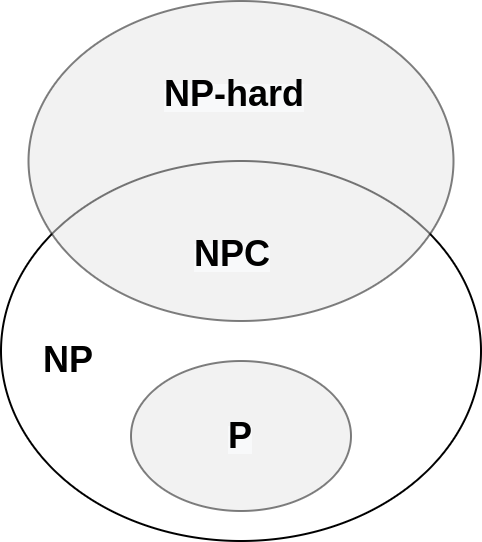
\includegraphics[width=0.4\linewidth]{img/npc.png}
    \caption{\label{fig:np}Illustration of the most common view of the P, NP, NPC, and NP-hard relationship. Adapted from Cormen et al. (2009) \cite{cormen2009introduction}.}
\end{figure}

As stated, it is considered unlikely that \gls{MILP} problems can be solved in polynomial time. Therefore, it is more fruitful to improve upon the best existing solution algorithms and evaluating the improvements on practical problems. As the improvements attempted by substituting variable selection algorithms do not affect the running time complexity of the \gls{BnB} algorithm, this will not be discussed.  










\section{Branch and Bound}\label{sec:back_bnb}

A \textit{relaxation} of a \gls{MILP} problem is achieved by relaxing the integrality constraint, as shown in \Cref{fig:milpfig}. Obtaining the solution to the relaxed problem gives a lower bound on the optimal solution (for a minimization problem). Naturally, any feasible solution to the integrality-constrained problem gives an upper bound to the solution. Furthermore, if the solution to the relaxed problem adheres to the integrality constraints, it is also the solution to the \gls{MILP} problem \cite{wolsey2020integer}.






The most prevalent solution algorithm for \gls{MILP} problems exploits these results, by sequentially dividing the solution space until the optimum with the integrality constraint is found. This is done by branching in a bipartite graph according to \cite{gasse2019exact}:
\begin{align} \label{eq:branch}
    x_{i} \leq\left\lfloor x_{i}^{\star}\right\rfloor \vee x_{i} \geq\left\lceil x_{i}^{\star}\right\rceil, \quad \exists \; i \leq p \mid x_{i}^{\star} \notin \mathbb{Z}    
\end{align}
Further creating sub-problems with this binary decomposition. A general algorithm for this process is presented in \Cref{alg:bnb}, and an illustration of this process is shown in \Cref{fig:bandb1}.

\begin{algorithm}[H]
    \SetAlgoLined
    \KwResult{Optimal point and solution value of given problem.}
    Set $L = \{X\}$ and initialize $\hat{x}$\; 
    \While{$L \neq \emptyset $}{
        Select a subproblem $S$ from $L$ to explore\;
        \If{a solution $\hat{x}_* \in \{x \in S \;|\; f(x) < f(\hat{x})\}$ can be found}{
            Set $\hat{x} = \hat{x}_*$\;
        }
        \If{$S$ cannot be pruned}{
            Partition $S$ into $\{S_1, S_2 ..., S_r\}$\;
            Insert $\{S_1, S_2 ..., S_r\}$ into $L$\;
        }
        Remove  $S$ from $L$\;
    }
    Return $\hat{x}$\;
    \caption{\label{alg:bnb} A generic Branch and Bound algorithm \cite{morrison2016branch}.}
\end{algorithm}

%https://tex.stackexchange.com/questions/416359/branch-and-bound-tree-in-tikz
\comments{
\begin{figure}
\centering
\begin{forest}
  branch and bound,
  where level=1{
    set branch labels={x\leq}{}{x\geq}{},
  }{
    if level=2{
      set branch labels={}{\geq y}{}{\leq y},
    }{},
  }
  [1055.56:S:950
    [1000:S_1:950:5
    ]
    [1033:S_2:950:6
      [1033:{S_2,1}:950:1]
      [950:{S_2,2}:1033:2]
    ]
  ]
\end{forest}
\caption{\label{fig:bandb1}Illustration of the branch and bound algorithm}
\end{figure}}

\begin{figure}
    \centering
    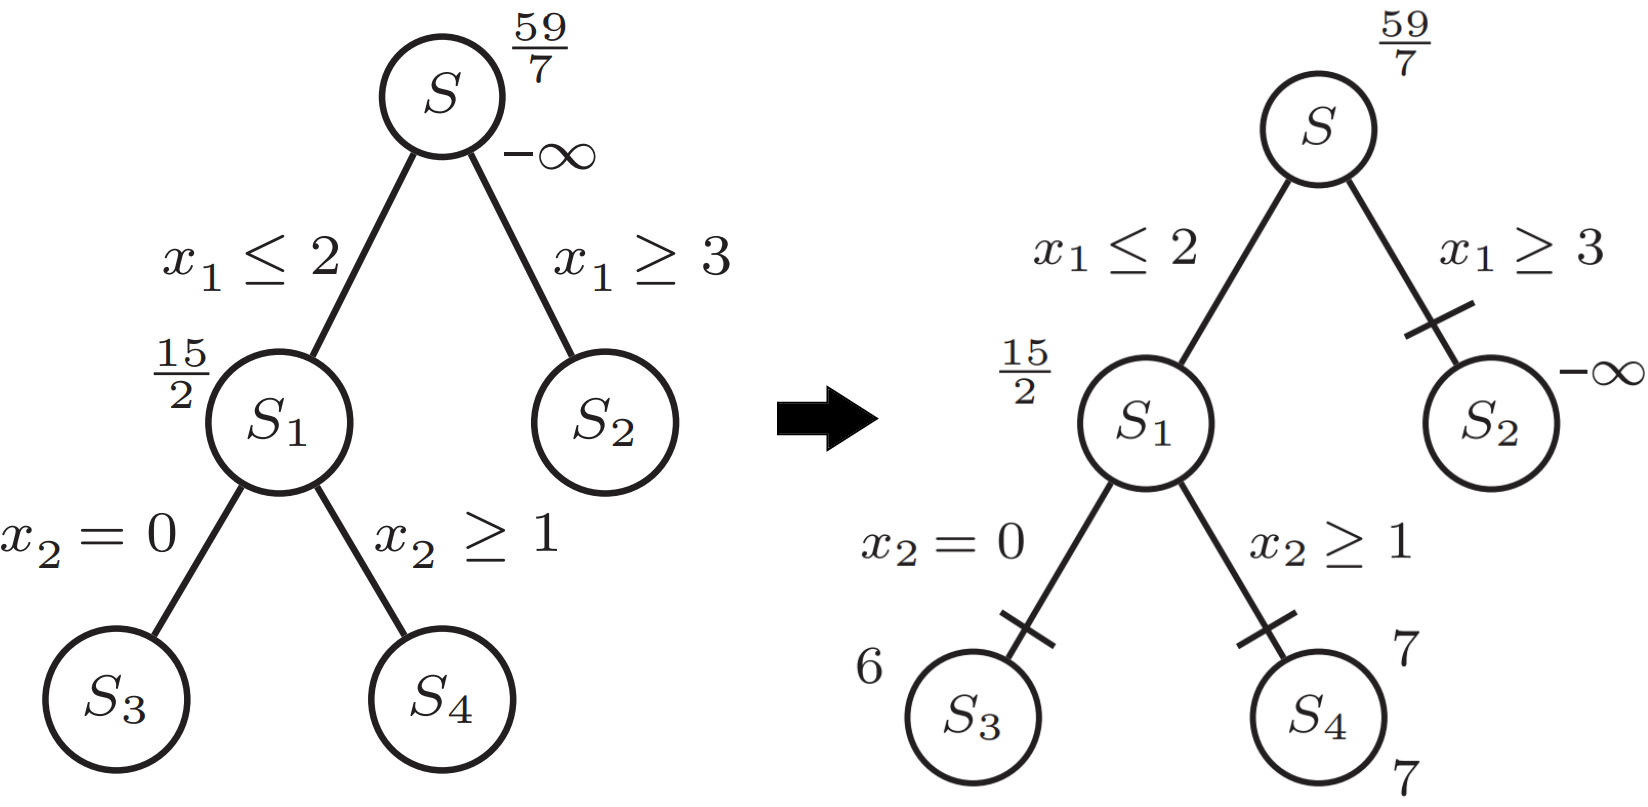
\includegraphics[width=0.8\linewidth]{img/bnb.png}
    \caption{\label{fig:bandb1}Illustration of the branch and bound algorithm adapted from a maximization problem in \textit{Integer Programming }(2020) \cite{wolsey2020integer}}
\end{figure}

For each generated solution, represented by nodes in \Cref{fig:bandb1}, a relaxation of the problem is solved in order to obtain an upper and lower bound on the solution of the sub-problem. 
These values are shown on the top and bottom right, respectively. 
Generating upper and lower bounds for solutions allows for discarding a large number of solutions \cite{wolsey2020integer}. Branches can be \textit{pruned} (meaning no further partitioning from that branch) if they meet at least one of the following three criteria \cite{wolsey2020integer}:
\newpage
\begin{enumerate}[label=(\roman*)]
    \item Pruning by optimality: $Z^t = \{\max \bm{c}^{\top} \bm{x} : \bm{x} \in S_t\}$ has been solved.
    \item Pruning by bound: $\overline{Z}^t \leq \underline{Z}^t$.
    \item Pruning by infeasiblity: $S_t = \emptyset $.
\end{enumerate}
For \Cref{fig:bandb1}, the graph on the right represents the tree after solving the relaxation, resulting in $S_2$ being pruned by infeasibility, $S_3$ cut off by bound and $S_4$ pruned by optimality.


The choice of node and variable to branch on to find the optimum in the fewest number of branching processes is central to an efficient implementation of \gls{BnB}. Partitioning the feasible set such that the node with the optimal value (criteria i) is found in the fewest possible branchings is the optimal strategy. 


\subsection{Valid Inequalities}\label{ssec:inequalities}

Another important method used in \gls{BnB} algorithms is the concept of valid inequalities. A valid inequality is an inequality that does not remove feasible solutions of the non-convex solution set but can remove potential solutions to the relaxed problems. A valid inequality can be expressed as:
\begin{equation}\label{eq:cut}
    \bm{\pi}^{\top} \bm{x} \leq \pi_0 \quad \forall \; \mathbf{x} \in  \bm{X}   
\end{equation}
where $\bm{X}$ is the feasible set as described in \Cref{eq:milp}. These inequalities reduce the size of the feasible set for the relaxations of the problem without removing feasible solutions of the original problem. An illustration of an \gls{ILP} with an added valid inequality is shown in \Cref{fig:cut}. Here the feasible set of the relaxation is reduced in size by the added constraint, while the feasible points of the \gls{ILP} remain feasible after the application of the inequality, as is given in \Cref{eq:cut}.

\begin{figure}
    \centering
    \begin{tikzpicture}[
        thick,scale=0.5, 
        every node/.style={scale=0.2}
        every path/.style = {},
        every node/.append style = {font=\sffamily}
      ]
      \begin{scope}
        \shade[right color=gray, left color=white, opacity=0.7]
          (-0.5,-0.5) rectangle (0,6.5);
        \shade[top color=gray, bottom color=white, opacity=0.7]
          (-0.5,-0.5) rectangle (8.5,0);
        \shade[left color=gray, bottom color=gray, right color=white, opacity=0.5]
          (-0.5,5.5) -- (8.5,3) -- (8.5,6.5) -- (-0.5,6.5) -- cycle;
       \shade[left color=gray, right color=gray, opacity=0.5]
         (2.5,6.5) -- (8.5,6.5) -- (8.5,0) -- (5,0) -- cycle;
        \draw[->] (-0.5,0) -- (8.5,0) node[below] {x};
        \draw[->] (0,-0.5) -- (0,6.5) node[above] {y};
        \foreach \i in {0,1,...,6.5} {
          \draw[help lines] (-0.5,\i) -- (8.5,\i);
        }
        \foreach \i in {2,4,...,8.5} {
          \draw[help lines] (\i,6.5) -- (\i,-0.5);
        }
        \foreach \i in {0,1,...,5} {
          \node[draw,cross out] at (0,\i) {};
        }
        \foreach \i in {0,1,...,4} {
          \node[draw,cross out] at (2,\i) {};
        }
        \foreach \i in {0,1,...,2} {
                \node[draw,cross out] at (4,\i) {};
        }
      \end{scope}
      \draw[very thick, ->] (9,3.25) -- node[above, text width=3cm, align=center]
        {} (11.5,3.25);
      \begin{scope}[shift={(13,0)}]
        \shade[right color=gray, left color=white, opacity=0.7]
          (-0.5,-0.5) rectangle (0,6.5);
        \shade[top color=gray, bottom color=white, opacity=0.7]
          (-0.5,-0.5) rectangle (8.5,0);
        \shade[left color=gray, bottom color=gray, right color=white, opacity=0.5]
          (-0.5,5.5) -- (8.5,3) -- (8.5,6.5) -- (-0.5,6.5) -- cycle;
        \shade[left color=gray, right color=gray, opacity=0.5]
          (2.5,6.5) -- (8.5,6.5) -- (8.5,0) -- (5,0) -- cycle;
        \shade[left color=gray, right color=gray, opacity=0.5]
          (0.0,6.5) -- (8.5,6.5) -- (8.5,0) -- (6.0,0) -- cycle;
        \draw[->] (-0.5,0) -- (8.5,0) node[below] {x};
        \draw[->] (0,-0.5) -- (0,6.5) node[above] {y};
        \foreach \i in {0,1,...,6.5} {
          \draw[help lines] (-0.5,\i) -- (8.5,\i);
        }
        \foreach \i in {2,4,...,8.5} {
          \draw[help lines] (\i,6.5) -- (\i,-0.5);
        }
        \foreach \i in {0,1,...,5} {
          \node[draw,cross out] at (0,\i) {};
        }
        \foreach \i in {0,1,...,4} {
          \node[draw,cross out] at (2,\i) {};
        }
        \foreach \i in {0,1,...,2} {
                \node[draw,cross out] at (4,\i) {};
        }
      \end{scope}
    \end{tikzpicture}
    \caption{Figure of \Gls{ILP} before and after an added valid inequality.}
    \label{fig:cut}
\end{figure}
 


Algorithms that find these inequalities during the \gls{BnB} algorithm are called \textit{Branch and Cut}. The nomenclature comes from calling the application of these inequalities \textit{cuts} or \textit{cutting planes}.
When an application of inequalities are only employed on the root node (before dividing the solution space in the enumeration), the algorithm is sometimes referred to as \textit{Cut and Branch} rather than \textit{Branch and Cut} \cite{wolsey2020integer}.






\subsection{Primal and Dual Heuristics}

The modern implementations of \gls{BnB} solvers base their efficiency on the implementation of \textit{heuristics} \cite{khalil2020towards}, which are divided into the classes \textit{primal} and \textit{ dual}. Heuristic is synonymous with "human-designed rule" in this context.

\textit{Primal heuristics} are methods for finding feasible solutions at a given \gls{BnB} node, where the quality, i.e. the distance to the optimal bound, is the determining factor to whether the feasible solution is useful or not \cite{khalil2020towards}. These heuristics are as costly as they are useful, and modern solvers periodically run different heuristics at different times during the solution process \cite{khalil2020towards}.

\textit{Dual heuristics} are the methods that find the lower bound of the optimization problem. This includes solution of relaxations of the problem as well as the addition of valid inequalities. 

Quoting Khalil (2020) \cite{khalil2020towards}:
\begin{quote}
    [...] the
primal side refers to the quest for good feasible solutions, whereas the dual side refers to
the search for a proof of optimality.
\end{quote}






\subsection{Branching Variable Selection Strategy}\label{ssec:branchingstrategy}

As mentioned, an important decision in the \gls{BnB} algorithm is the choice of the variable that should be branched on. 
There exists many heuristics for solving this, which vary in computational complexity and accuracy. 
A good branching algorithm should choose to branch on variables that lead to small solution trees (fewer nodes evaluated) and find these variables in a computationally efficient manner. 

The current branching strategy resulting in the smallest solution trees is known as \textit{Strong Branching} (\gls{SB}) \cite{applegate1995finding}, and the application of this branching strategy at every node is known as \textit{Full Strong Branching} (\gls{FSB}) \cite{achterberg2004branching}. 
This branching policy is based on determining the best variable to branch on by solving the relaxation for every candidate variable and is therefore very computationally expensive compared to other methods \cite{achterberg2004branching}.

All popular variable selection strategies depend on scoring all the possible variables and selecting the variable with the most optimal score \cite{achterberg2004branching}. There are two other common classes of branching strategies than \gls{FSB}: \textit{Most Infeasible Branching} (\gls{MIB}), where the variable with the fractional part of the relaxation optimum closest to $0.5$ is selected (a very poor policy) 
and \textit{Pseudo-cost Branching} (\gls{PC}), which relies on the expected change in objective value based on previous branching on the variable in question
\cite{achterberg2004branching}. Today, combinations of \gls{FSB} and \gls{PC} are most common \cite{anand2017comparative}.   

In the literature, the branching strategy is referred to as a strategy, policy, or rule, in this project \textit{policy} is used.  








\subsection{Learned Branching Policy}

Recently, attempts have been made to find a branching strategy based on statistical learning. 

Using machine learning, specifically imitation learning, to find good candidate variables for branching in a less computationally demanding manner was proposed by Elias Khalil \cite{khalil2016learning}. Various methods for learning in branching include \textit{ Support Vector Machine Ranking} (\Gls{SVM}) \cite{khalil2016learning}, \textit{Graph Convolutional Neural Networks} (\gls{GCNN}) \cite{gasse2019exact} and \textit{Feature-wise Linear Modulation} (\gls{FiLM}) \cite{gupta2020hybrid}.

The fundamental assumption to this approach is that a computationally efficient approximation to the most computationally demanding but most accurate branching policy can be learned. The algorithm will use imitation learning on the branching expert to find a computationally less expensive non-linear function approximation to the expert algorithm's variable scoring. Then, the algorithm branches on the variable with the highest score. 
%This can be expressed as: 
%\begin{align}
%    f(i) &=  \pi_{SB} (i) + \epsilon \quad \forall \; i \in \mathcal{C}\\
%    f(i) &= s_i\\
%    i^*_f &= \underset{i \in \mathcal{C}}{\mathrm{argmin}} \; \bm{s}_i
%\end{align}
%where $f$ is the learned function, $\mathcal{C}$ is the set of possible branching variables, $\pi_{SB}$ is the Strong Branching strategy and $\epsilon$ is the deviation in the scoring function. 




\section{Markov Decision Processes}\label{sec:back_mdp}

This section presents the \textit{Markov Decision Process} formulation of the variable selection problem. 


\subsection{Markov Decision Processes Formulation}\label{ssec:mdp}

Central to the advancement of learned strategies in \gls{BnB} is the interpretation of the solution algorithm as an \textit{agent} in a \textit{Markov Decision Process} (\gls{MDP}) \cite{gasse2019exact}. This interpretation relates the problem to a large collection of literature on the topic \cite{howard1960dynamic}.

The agent is at time $t$ in a state $\mathcal{S}_t$, from which it performs an action $\mathcal{A}_t$ that transforms the agent to the state $\mathcal{S}_{t+1}$ and receives the \textit{reward} $\mathcal{R}_{t+1}$ \cite{prouvost2021ecole}. The probability of an agent performing action $a$ in state $s$ is given as $\pi (a | s)$. The probability distribution for the agent for the agent to transition to a new state $s'$ is given as $\mathbb{P}(s', r | a, s)$ \cite{prouvost2021ecole}. 

 
A sequence of actions generates a sequence of trajectories $\tau$, and is described as an \textit{episiode}. The probability of a trajectory is given in Prouvost et al. (2021) \cite{prouvost2020ecole} as:
\begin{equation}
    \mathbb{P}(\tau) \sim \underbrace{\mathbb{P}(\mathcal{S}_0)}_{\text{initial state}}
\prod_{t=0}^\infty \underbrace{\pi(\mathcal{A}_t | \mathcal{S}_t)}_{\text{next action}}
\underbrace{\mathbb{P}(\mathcal{S}_{t+1}, \mathcal{R}_{t+1} | \mathcal{A}_t, \mathcal{S}_t)}_{\text{next state}}
\end{equation}

These definitions now allow a formulation of the \gls{MDP} control problem, which is the problem of interest in this thesis. The control problem consists of finding the action policy that maximizes the reward. %, and can be stated as: 
%\cite{prouvost2020ecole}
%\begin{equation}\label{eq:mdprcontrol}
%    \pi^\star = \underset{\pi}{\operatorname{arg\,max}}
%\lim_{T \to \infty} \mathbb{E}_\tau\left[\sum_{t=0}^{T} %\mathcal{R}(\mathcal{S}_t)\right]
%\end{equation}



\subsection{Partially-observable Markov Decision Processes}

A subset or generalization of an \gls{MDP} is the \textit{Partially-observable Markov Decision Process }(\gls{PO-MDP}) \cite{monahan1982state}. Processes of this class allows for uncertainty of the states as well as additional acquisition of state information \cite{monahan1982state}. The agent will therefore decide actions based on the observation of the state, given as $\mathcal{O}$ \cite{prouvost2021ecole}. All past observations of the observations, rewards and actions are given in the history $H_t$, given as \cite{prouvost2021ecole}:
\begin{equation}
    H_t = \{\mathcal{O}(\mathcal{S}_0), \mathcal{R}(S_0), \mathcal{A}_0, ..., \mathcal{O}(\mathcal{S}_{t-1}), \mathcal{R}(S_{t-1}), \mathcal{A}_{t-1}, \mathcal{O}(\mathcal{S}_t)\}
\end{equation}
The generalization from \gls{MDP} to \gls{PO-MDP} concedes the Markovian nature of the trajectories \cite{prouvost2020ecole}.

In addition, the initial state is given by the distribution of the problem instance $I$, giving the relation $\mathbb{P}(\mathcal{S}_0) = \mathbb{P}(I) \mathbb{P}(\mathcal{S}_0 | I)  $\cite{prouvost2021ecole}. 

This results in the final formulation \cite{prouvost2021ecole}:
\begin{equation}
    \mathbb{P}(\tau) \sim \underbrace{ \mathbb{P}(I) \mathbb{P}(\mathcal{S}_0 | I)  }_{\text{initial state}}
\prod_{t=0}^\infty \underbrace{\pi(\mathcal{A}_t | H_t)}_{\text{next action}}
\underbrace{\mathbb{P}(\mathcal{S}_{t+1}, \mathcal{R}_{t+1} | \mathcal{A}_t, \mathcal{S}_t)}_{\text{next state}}
\end{equation}

An illustration of the Markov Decision Process control loop from the documentation of \gls{Ecole} is shown in \Cref{fig:mdp}.

\begin{figure}
    \centering
    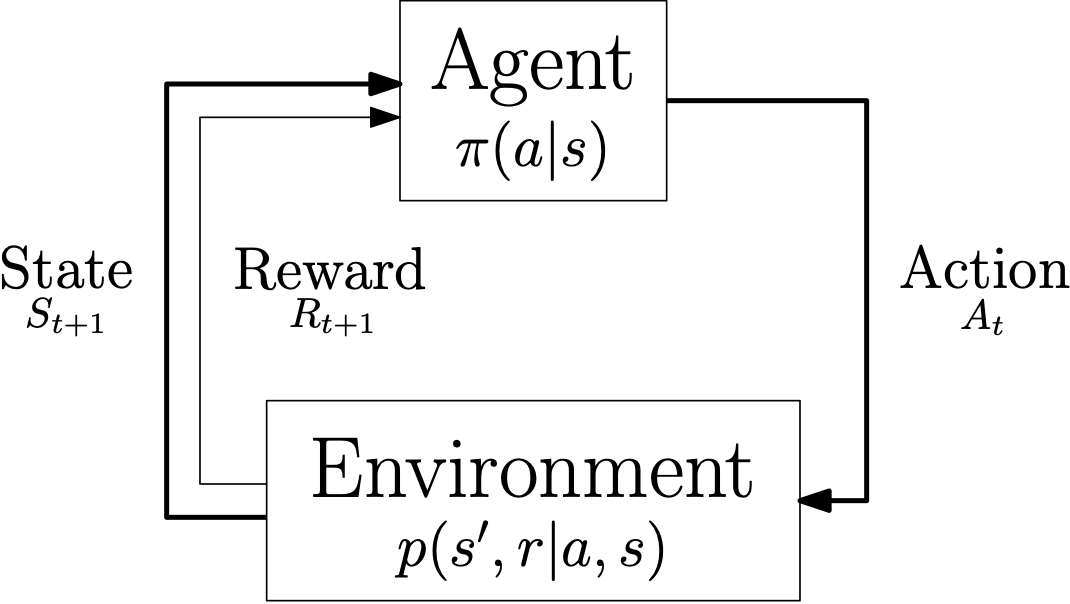
\includegraphics[width=0.55\linewidth]{img/mdp.png}
    \caption{Illustration of the Markov Decision Process control loop. Figure from Provoust et al. (2021) \cite{prouvost2021ecole}.}
    \label{fig:mdp}
\end{figure}



\subsection{Branch \& Bound as a PO-MDP}\label{ssec:pomdp}

Interpreted in the language of \gls{MDP}s, the \gls{BnB} algorithm is the \textit{environment} and a concrete \gls{MILP} problem instance is an \textit{episode} in this environment. The \textit{agent} is the brancher, where in this thesis the variable selection policy is the component of interest, ignoring the node selection policy. The state of the solver consists of the \gls{BnB} tree at that instance, as well as the observations at each node (the \textit{history} of the \gls{PO-MDP}).

This formulation is the basis for the \textit{Ecole} framework, which is discussed in \Cref{ssec:ecole}
The \gls{PO-MDP} formulation allows for the agent in the \gls{BnB} environment to be learned through \textit{reinforcement learning}



\subsection{Branch \& Bound Observation}\label{ssec:obs}

A prerequisite for learning in \gls{BnB} is the observation of the state of the episode, i.e. the state of the solver of an instance at a specific node in the solution tree. 

Little attention towards these features are found in the major publications in this field (\cite{gasse2019exact,gupta2020hybrid}), however the observation is the foundation of the learning process.
\textit{Learning to Branch} by Khalil et al. (2016) \cite{khalil2016learning} contains multiple additional features, however these will not be discussed in this thesis. 

The features are divided into three classes: Variable features, constraint features and edge features.


\textbf{Variable Features}

For a candidate branching variable, relevant features include the type of the variable (binary, integer etc.), whether the variable has a defined lower and/or upper bound, and whether the solution is at at either of these bounds.  
If not, the variable has a fractionality that represents the solution of the relaxed problem.
At the solution node, the incumbent has a value that can be compared to incumbents at other nodes, as well as the relative impact of the variable on the objective value in the incumbent. 
The variable also has a state with respect to the solution of the relaxation with simplex --- if the variable is a basic or non-basic variable or other information relating to this solution.
Presented in Khalil et al. (2016) \cite{khalil2016learning} are also a number of other features that will not be utilized in this work.




\textbf{Constraint Features}

The cosine similarity represents a coefficient of the angle between the variable and the constraint.   
The bias of the constraint is also included. 
An additional feature is whether the variable is at the constraint in the relaxation
Each constraint also has a value from the solution of the dual problem. 


\textbf{Edge Features}

The edge features consist of the constraint coefficient, meaning the coefficient that is multiplied with the candidate variable.




\subsection{Bipartite Graph Representation}

The application of \gls{GCNN}s on \gls{MILP} and sub-\gls{MILP} problems rely on the bipartite representation of constraints and variables as presented in Gasse et al. (2019) \cite{gasse2019exact}.
This concept will be introduced with an example \gls{MILP} given as:
\begin{align}\label{eq:bipex}
    \min \quad &\texttt{v}_1 + \texttt{v}_2 + \texttt{v}_3\\ 
    s.t. \quad &\texttt{v}_1 + \texttt{v}_2 - \texttt{v}_3 \geq 1 \qquad (c_1)\nonumber\\
    &\texttt{v}_3 \geq \frac{1}{2}\qquad\qquad\quad\;\,\; (c_2)\nonumber\\
    &\mathbf{v} \in \mathbb{B}^N \nonumber
\end{align}

\begin{figure}
    \centering
    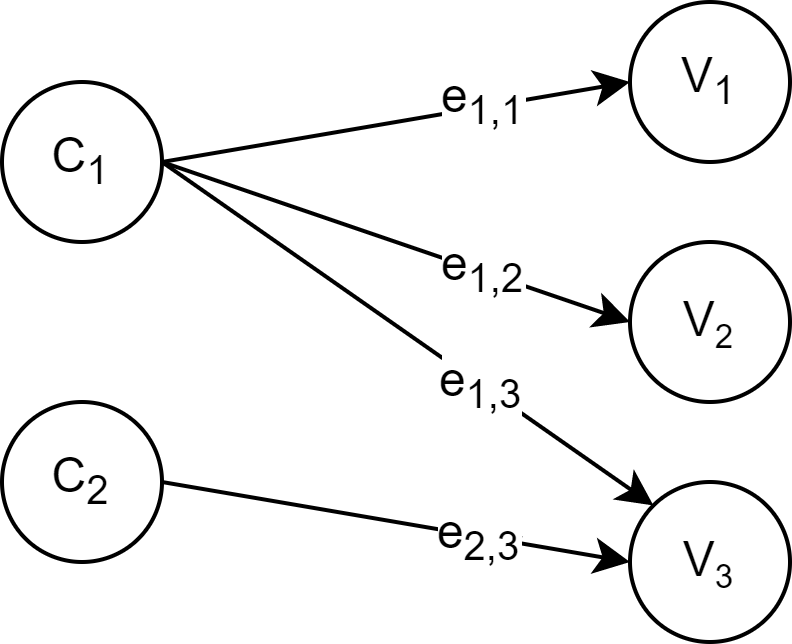
\includegraphics[width=0.40\linewidth]{img/bipartite_zoom.png}
    \caption{Example of a bipartite constraint-variable graph.}
    \label{fig:bipartite_cv}
\end{figure}

For \Cref{eq:bipex}, the corresponding constraint-variable graph representation can be illustrated as in
\Cref{fig:bipartite_cv}.

Constraints and variables are the numbered nodes of the graphs, while the edges represent the relation between the nodes. 



\section{Machine Learning Models}\label{sec:back_models}


The \gls{ML}-models used in the thesis are presented in this section. Firstly the Multi-Layer Perceptron and Graph Convolutional Neural Network models, before the concepts of \textit{Ablation studies} and \textit{Reinforcement Learning} are given.

\subsection{Multi-layer Perceptrons}\label{ssec:back_mlp}

Multi-Layer Perceptrons (\gls{MLP}s), more commonly known as deep feed-forward neural networks, are recommended by Gupta et al. (2020) \cite{gupta2020hybrid} as a less computationally expensive alternative to the approaches by Khalil et al. (2016) \cite{khalil2016learning} and Gasse et al. (2019) \cite{gasse2019exact}. 

\gls{MLP}s are networks that generate a nonlinear function $y = f(\mathbf{x}; \bm{\theta})$, where $x$ is the input $y$ is the output and $\bm{\theta}$ represents the parameters of the function. The parameters are learned during repeated optimization, and will under ideal circumstances converge to approach the goal function $y = f^*(\mathbf{x})$. The function is realized as a series of compositions of functions. The composed functions are represented as an acyclical, directed graph \cite{nielsen2018neural}, and can be expressed as:
\begin{align}
    y = f_L \circ f_{L-1} \circ \ldots \circ f_{1} \circ f_{0} (\mathbf{x})  
\end{align}
The functions are denoted as layers of the perceptron, and are implemented as affine functions of every input parameter at every node, $\mathbf{z}_l = \mathbf{x}_{l-1}^T \mathbf{w}_l + \mathbf{b}_l$. Applying non-linear function, known as an \textit{activation function}, allows the \gls{MLP} to represent arbitrary nonlinear functions \cite{goodfellow2016deep}. This is expressed as $\mathbf{x}_l = \mathbf{a}(\mathbf{z}_l)$.

The computation of the output of the function given its input is known as a \textit{forward pass} through the network. The required computations for a single input vector into a network with $ n $ hidden layers will include $ n + 1 $ matrix multiplications and $ n + 1 $ applications of the non-linear activation function, given that there is an activation function on the output. 

Depending on the training configuration, the problem can be interpreted as a classification problem or regression problem (or a ranking problem, as in \cite{khalil2016learning}). In the following experiments, the former approach is selected, as has become popular after Gasse et al. (2019) \cite{gasse2019exact}. 










\subsection{Graph Convolutional Neural Networks }

Graph Convolutional Neural Networks (\gls{GCNN}s) is a term for neural networks that have input data represented in a graph-structure that is processed by the convolution operation \cite{kipf2016semisupervised}. In this thesis, the terms \gls{GCNN} and \gls{GNN} will be used interchangeably. The graph convolution operation is defied by the propagation rule \cite{kipf2016semisupervised}:
\begin{equation}
    H^{(l+1)} = \sigma \left( \Tilde{D}^{-\frac{1}{2}} \Tilde{A} \Tilde{D}^{-\frac{1}{2}} H^{(l)}W^{(l)}\right)
\end{equation}
where $H^{(l)}$ is the matrix of activations in layer $l$. $\Tilde{A} = A + I_N$, where $A$ is the adjacency matrix representing the undirected graph $\mathcal{G}$, and $\Tilde{D} = \sum_j \Tilde{A}_{i j}$. $\sigma( \cdot) $ is a nonlinear activation function.
This operation is shown to be inspired by the first-order approximations to spectral filters on graphs \cite{kipf2016semisupervised}.

The term \textit{embeddings} will be used in this thesis for continuous-variable representations derived from the input features, as it is used in Gasse et al. (2019) \cite{gasse2019exact}. 





Models that leverage the graph nature of combinatorial optimization problems have been shown to have satisfactory performance, see e.g. Dai et al. (2018) \cite{dai2018learning}. 
\gls{GCNN}s are proposed by Gasse et al. \cite{gasse2019exact} as an alternative to the feature-rich approaches by Khalil et al. (2016) \cite{khalil2016learning}. 
The application of \gls{GCNN}s on \gls{BnB} algorithms rely on the bipartite graph structure that results from the solution process, as explained in \Cref{sec:back_bnb}. At each point before the variable selection process, the state of the solution algorithm graph can be processed by the \gls{GCNN} algorithm. 

The state of the \gls{BnB} graph at a node can be represented as $s_t = (\mathcal{G}, \mathbf{C}, \mathbf{E}, \mathbf{V})$, where $\mathcal{G}$ represents the bipartite \gls{BnB} solution graph at that time instance, $\mathbf{C}$ represents the constraints, $\mathbf{E}$ represents the \textit{edges}, or connections between the variables and constraints, and $\mathbf{V}$ represents candidate variables.  

Gasse et al. (2019) \cite{gasse2019exact} presents three motivating points for why graph convolutions would be a good architecture for learning to branch:
\begin{enumerate}[label=(\roman*)]
    \item They are well-defined no matter the input graph size.
    \item Their computational complexity is directly related
to the density of the graph, which makes it an ideal choice for processing typically sparse \gls{MILP}
problems.
    \item They are permutation-invariant, that is they will always produce the same output no
matter the order in which the nodes are presented.
\end{enumerate}






\subsection{Ablation Studies}

The concept of ablation studies in machine learning, as presented in 
Meyes et al. (2019) \cite{meyes2019ablation} is presented in this section.
Ablation studies hail from the field of neuroscience, in which a complex system, e.g. the brain, is examined after removing different sections. The function of the removed sections can then be inferred by the change in the observed reaction to external stimuli \cite{meyes2019ablation}.

In the context of \gls{ML}, ablation studies are a formalization of observing changes in performance after the removal of components of artificial neural networks \cite{meyes2019ablation}.  
The concept, or at least the formalization, is not yet considered a standard method in \gls{ML} research \cite{sheikholeslami2019ablation}.
In this thesis, the concept of an ablation study will be interpreted more broadly than in Meyes et al. (2019) \cite{meyes2019ablation}, as the networks in this thesis are retrained after each section is removed. This form of ablation study is coined as \textit{model ablation} in Sheikholeslami (2019) \cite{sheikholeslami2019ablation}.





\subsection{Reinforcement Learning}

The subset of machine learning described as Reinforcement Learning (\gls{RL}) is highly relevant in the context of \gls{ML} in \gls{CO}. No results will be discussed in this thesis, however, a background in the topic is necessary to understand both other works in the field and the long-term goals of the project.

\gls{RL} encompasses the problem of an \textit{agent} learning a \textit{policy} for behaving in an \textit{environment} so as to achieve a global objective. Any sequential decision-making problem with a measure of optimality that relies on past experience can be formulated as a \gls{RL} problem \cite{francois2018introduction}. In addition, the approach has seen success in a number of fields in the past years with the integration of deep learning models, often termed deep \gls{RL} \cite{francois2018introduction}. Most notable of the advancements might be AlphaZero, Google's successful chess-AI \cite{silver2017mastering}. \gls{RL} has the important property of being independent of data, meaning a number of core \gls{ML} challenges (quantity, quality, and bias of data) are rendered irrelevant. 

\gls{RL} is particularly interesting in \gls{BnB} because of the \gls{MDP} nature of the algorithm, and the assumption that the handcrafted heuristics and sub-algorithms prevalent in modern solvers are either inefficient or inaccurate compared to the theoretical capabilities of, i.e. neural networks. 

Many attempts have been made at implementing \gls{RL} in \gls{CO}, see for example Etheve et al. (2020) \cite{etheve2020reinforcement} or Tang et al. (2020) \cite{tang2020reinforcement}. Approaches for learning variable selection, such as reported in Scavuzzo (2020) \cite{scavuzzo2020learning}, rely on efficient and accurate pre-trained models based on imitation learning, like the models presented in this thesis. More knowledge is likely needed for the pure \gls{RL} approach to take over the mantle.
\footnote{Attempts on \gls{RL} models were also made by the author of this thesis, but the models did not prove useful with the chosen method and are therefore not reported.}
Cappart et al. (2021) \cite{cappart2021combinatorial} also conclude that useful \gls{RL} policies are not mature yet. 

\chapter{Methods}\label{cha:methods}

In this chapter, the selected methods for the experiments are presented and discussed.  
An understanding of the theoretical groundwork of the project from \Cref{cha:background} is assumed. A substantial part of the methods are taken directly or indirectly from the source code of Gasse et al. (2019) \cite{gasse2019exact}, Gupta et al. (2020) \cite{gupta2020hybrid}, and the \gls{Ecole} source code \cite{prouvost2020ecole}. Some sentences and formulations are adapted from the project report \textit{Multi-layer Perceptrons for Branching in Mixed-Integer Linear Programming} (2020), as this thesis shares methods with the aforementioned report. 


\section{Dataset}\label{sec:dataset}

This section presents the selected data set and the process of generating trainable and testable data for the models. 
This will include a presentation of the problem instances, the generation of the expert solutions as well as the features that will be the input of the \gls{ML} models. 



\subsection{Problem Instances}\label{ssec:probleminstances}

In order to evaluate the methods presented in this project to the previous advances in the field, artificially generated \gls{MILP} problems found in Gasse et al. (2019) \cite{gasse2019exact} are used to train and evaluate the models. These problems are also the standard implemented in \gls{Ecole}.
The problems are expressed as pure binary programs. The results of the algorithm are, however, generalizable to general \gls{MILP} problems, as it extends the general \gls{BnB} algorithm \cite{gasse2019exact}. 

In the mentioned articles, four problem classes are used: set covering, combinatorial auctions, capacitated facility location, and maximum independent set. In this thesis, only the first two will be used due to problems in the \gls{Ecole} framework that have since been resolved. 

%Problems are generated in three sizes: small, medium, and large. Small instances are used for training, while medium and large problem sizes are reserved for evaluating the extended algorithm's ability to generalize on more challenging problems. These problem sizes represent what current algorithms can solve within seconds (for the small instances) and multiple minutes (for the large instances).


\textbf{Set Covering}

The set covering problem is implemented in \gls{Ecole} as described in Balas \& Ho (1980) \cite{balas1980set} \footnote{The available version of this paper contains nearly illegible equations, the article Minoux (1987) \cite{minoux1987class} has therefore been used to supplement.}. The general problem includes a set of vertices $V_j$ and a matrix of costs $c_j$ for activating an edge between any two vertices. The activation of an edge is modeled with the binary variable $x_j$ and the characteristic vector of subset $V_j$ denoted $\textbf{A}_j$. The binary linear problem of covering all vertices at minimum cost can be expressed as \cite{minoux1987class}: 
\begin{align}
    \min &\sum_{i=1}^N c_i x_i \\ s.t. \; &\sum_{i=1}^N \mathbf{A}_i x_i \leq \mathbf{1} \\
    \mathbf{x} &\in \mathbb{B}^N 
\end{align}
The problem is therefore a pure binary linear problem with only inequality constraints. The set covering problem is a well-known class and is one of Karp's 21 \gls{NP}-complete problems \cite{karp1972reducibility}.  

\textbf{Combinatorial Auction}

The combinatorial auction problem is the problem with the shortest solution time in the mentioned articles \cite{gasse2019exact,gupta2020hybrid}. The problem is implemented by Gasse et al. (2019) \cite{gasse2019exact}, and is based on the formulation presented in Leyton-Brown et al. (2020) \cite{brown2000towards}. The version is specifically the \textit{arbitrary} formulation from the original article \cite{brown2000towards}. In this formulation, $N$ is the number of combinations of items, $p_i$ is the price of an item, $\mathcal{P}$ is the set of all items, and $a_{i,j} \in \mathbb{B}$ represents whether item $j$ belongs to combination $i$. With this, the problem can be stated as \cite{abrache2007combinatorial}:
\begin{align}
    \max &\sum_{i=1}^N p_i x_i \\ s.t. \; &\sum_{i=1}^N \mathbf{a}_{i,j} x_i \leq 1 \,, \quad \forall \, j \in \mathcal{P}\\ \mathbf{x} &\in \mathbb{B}^N 
\end{align}

The combinatorial auctions problem is based on multi-object auctions where bidders place monetary bids on bundles (combinations) of goods, and the optimization problem is to find the bids that maximize the profit of the auctioneer \cite{brown2000towards}. The problems are considered realistic and economically oriented, and are applicable to five broad domains in which optimization is important: Proximity in Space, Paths in Space, Arbitrary Relationships, Temporal Matching, and Temporal Scheduling \cite{brown2000towards}. The problems are \gls{NP}-hard \cite{dong2012combinatorial}. 

%\subsubsection{Capacitated Facility Location}


%\subsubsection{Maximum Independent Set}


%Barabasi-Albert graph.
%\footnote{In Gasse et al. (2019) the graph is reported to be of the type Erd\"{o}s-R\'{e}nyi, however the implementation is in fact a Barabasi-Albert graph.}




\subsection{Expert Solution Generation}\label{ssec:expertsolutiongeneration}

The generated problems are solved using the Full Strong Branching policy, as explained in \Cref{ssec:branchingpolicy}. To not interfere with branching policies, the application of cutting planes to the problem is restricted to the root node, before any branching decisions are made. This means that the Branch and Bound algorithm used in these experiments could be called a \textit{Cut and Branch} algorithm, as is discussed in \Cref{ssec:inequalities}.
However, without loss of generality and for simplicity, the algorithm will be referred to as \textit{Branch and Bound} in this thesis despite the initial application of cutting planes.  


\begin{algorithm}[H]
    \SetAlgoLined
    \KwResult{Variable selection samples}
    \For{$episode\in EPISODES$}{
        \While{episode not solved}{
            $\rho\leftarrow rand()$\;
            \eIf{$\rho \leq 0.05$}{
                $samples\leftarrow node\_ state$\;
                $scores\leftarrow SB\_scores$\;
                Save scores and state\;
                Branch on SB score\;
                }{
                Branch on pseudo-cost scores\;
            }
        }
    }
    
    \caption{\label{alg:datacol} Data collection algorithm}
\end{algorithm}


The algorithm for data collection is shown in \Cref{alg:datacol} and is adapted from Gasse et al. (2019) \cite{gasse2019exact}. During training, 5 \% of the branching variable decisions are done by the strong branching expert, compared to 5 \% in Gasse et al. (2019) \cite{gasse2019exact} and 100 \% in Gupta et al. (2020) \cite{gupta2020hybrid}. This method of generating expert samples has been criticized by Sun et al. (2021) \cite{sun2021improving}, among other reasons because strengths of \gls{SB} cannot be learned through variable selection only. The reader is referred to this article for further reading, in addition to the thesis Ross (2013) \cite{ross2013interactive} for more on expert imitation learning data. 



For every node, the \gls{SB} policy assigns a score to every possible branching variable. The best variable to branch on according to \gls{SB} is saved explicitly and then branched on. The best candidate variable is used for training, while the \gls{SB} scores are used for evaluating the learned policy. The placement of the selected variable compared to the candidate variables will be used to generate an accuracy score, to evaluate whether the algorithm is able to select among the top variables to branch on.  


\subsection{Branching Variable Features}

At nodes where the Strong Branching policy is used, available features for every possible branching variable is saved. The features, as explained in \Cref{ssec:obs}, are divided into the groups variable features, constraint features and edge features. These features are presented in 
 \Cref{tab:feats}. For a further explanation on the relevant features, see \Cref{ssec:obs}.
%
\renewcommand{\arraystretch}{1.5}
\begin{table}
	\centering
	\begin{tabular}{p{0.1\linewidth}p{0.2\linewidth}p{0.5\linewidth}}%{lll}
		\toprule
		  \textbf{Tensor} & \textbf{Feature} & \textbf{Description} \\ 
		  \toprule
		  \multirow{13}{*}{\textbf{V} (19)} & objective & Objective coefficient, normalized.  \\
		  & type (4) & Type (binary, integer, impl. integer, continuous) as a one-hot encoding. \\
		  & has\_lb & Lower bound indicator. \\
		  & has\_ub & Upper bound indicator \\
		  & reduced\_cost & Reduced cost, normalized. \\
		  & sol\_value & Solution value. \\
          & sol\_frac  & Solution value fractionality.\\
		  & sol\_is\_at\_lb & Solution value equals lower bound.\\
		  & sol\_is\_at\_ub & Solution value equals upper bound.\\
		  & scaled\_age & LP age, normalized. \\
          & inc\_val & Value in incumbent.\\
          & avg\_inc\_val & Average value in incumbents.\\
		  & basis\_status (4) & Simplex basis status (lower, basic, upper, zero) as a one-hot encoding.\\
		  \midrule
		  \multirow{5}{*}{\textbf{C} (5)} & obj\_cos\_sim & Cosine similarity with objective. \\
		  & bias & Bias value, normalized with constraint coefficients. \\
		  & is\_tight & Tightness indicator in LP solution. \\
		  & dualsol\_val & Dual solution value, normalized. \\
		  & scaled\_age & LP age, normalized with total number of LPs. \\
		  \midrule
		  \multirow{1}{*}{\textbf{E} (1)} & coef & Constraint coefficient, normalized per constraint. \\
		  %Static Features & 18 & Khalil et al. \cite{khalil2016learning} \\
		  %Dynamic Features & 54 & Khalil et al. \cite{khalil2016learning} \\
		% \addlinespace
		\bottomrule
	\end{tabular}
	\caption{Features of each variable in the data, adapted from Gasse et al. (2019) \cite{gasse2019exact}.}\label{tab:feats}
\end{table}
%
%The features of each node are saved as a custom python-class derived from the Data-class of pyTorch Geometric, and given in the source code of \textit{\gls{Ecole}}.


The underlying assumption is that these features are sufficiently correlated with the optimal variable to branch on, as it is given by the Strong Branching algorithm.
% math stuff here?



\section{Models}\label{sec:models}

This section presents the \gls{ML}-models used in the experiments. These models are \textit{iterative ablations} of the model presented in Gasse et al. (2019) \cite{gasse2019exact}, meaning each model is an increasingly simplified version of the original network. 


\subsection{Original Graph Convolutional Neural Network}\label{ssec:models_gcnn}

First, the nature of the Gasse GCNN has to be formulated. The central component is the graph convolution, which is modelled as two half-convolutions. This means that the convolution is divided into to subsequent passes --- one from variable to constraints and one from constraints to variables \cite{gasse2019exact}. 

The two half-convolutions can be expressed as \cite{gasse2019exact}:
\begin{equation}
    \mathbf{c}_i \leftarrow \mathbf{f}_{\mathcal{C}}\left( \mathbf{c}_i \; \sum_j^{(i,j) \in \mathcal{E}}\mathbf{g}_{\mathcal{C}} (\mathbf{c}_i, \mathbf{v}_j, \mathbf{e}_{i,j})\right), \qquad
    \mathbf{v}_j \leftarrow \mathbf{f}_{\mathcal{V}}\left( \mathbf{c}_j \; \sum_j^{(i,j) \in \mathcal{E}}\mathbf{g}_{\mathcal{V}} (\mathbf{c}_i, \mathbf{v}_j, \mathbf{e}_{i,j})\right)
\end{equation}
for all $i \in \mathcal{C}, j \in \mathcal{V}$. $\mathbf{f}_{\mathcal{C}},\mathbf{f}_{\mathcal{V}},\mathbf{g}_{\mathcal{C}},\mathbf{g}_{\mathcal{V}}$ are 2-layer perceptrons. 

The addition of the graph convolution operator results in the nodes of the bipartite variable-constraint graph containing information about its neighbors 

Gasse et al. (2019) \cite{gasse2019exact} also notes that it is common to normalize convolutional layers by the number of neighbors, however, they conclude that the loss of expressiveness by including this normalization is not beneficial. Therefore they include the affine normalization layer called a \textit{prenorm} layer. The layer is applied after the convolution, and is expressed as $ \mathbf{x} \leftarrow (\mathbf{x}-\bm{\beta})/\bm{\sigma}$. 

In the original implementation, the prenorm layer's coefficients ($\bm{\beta}, \bm{\sigma}$) are approximated and fixed in a pre-training phase, while the implementation in this thesis uses the new PyTorch library-component \verb|torch.nn.LayerNorm()|, where the coefficients are approximated continuously.     

After the normalizations, the features are transformed to \textit{embeddings} of a uniform size of 64 via a Multi-Layer Perceptron. 

An illustration of the Gasse \gls{GCNN} in given in \Cref{fig:gnn2}. The two convolutions are marked and the network layers are represented with a rectangle for each layer. The size of the hidden layers is consistently equal to 64. After the convolutions, a 2-layer perceptron transforms from the variable features (with information gained after the convolutions) to the single output. The dimensions for the tensors are marked in the figure. 
\begin{figure}
    \centering
    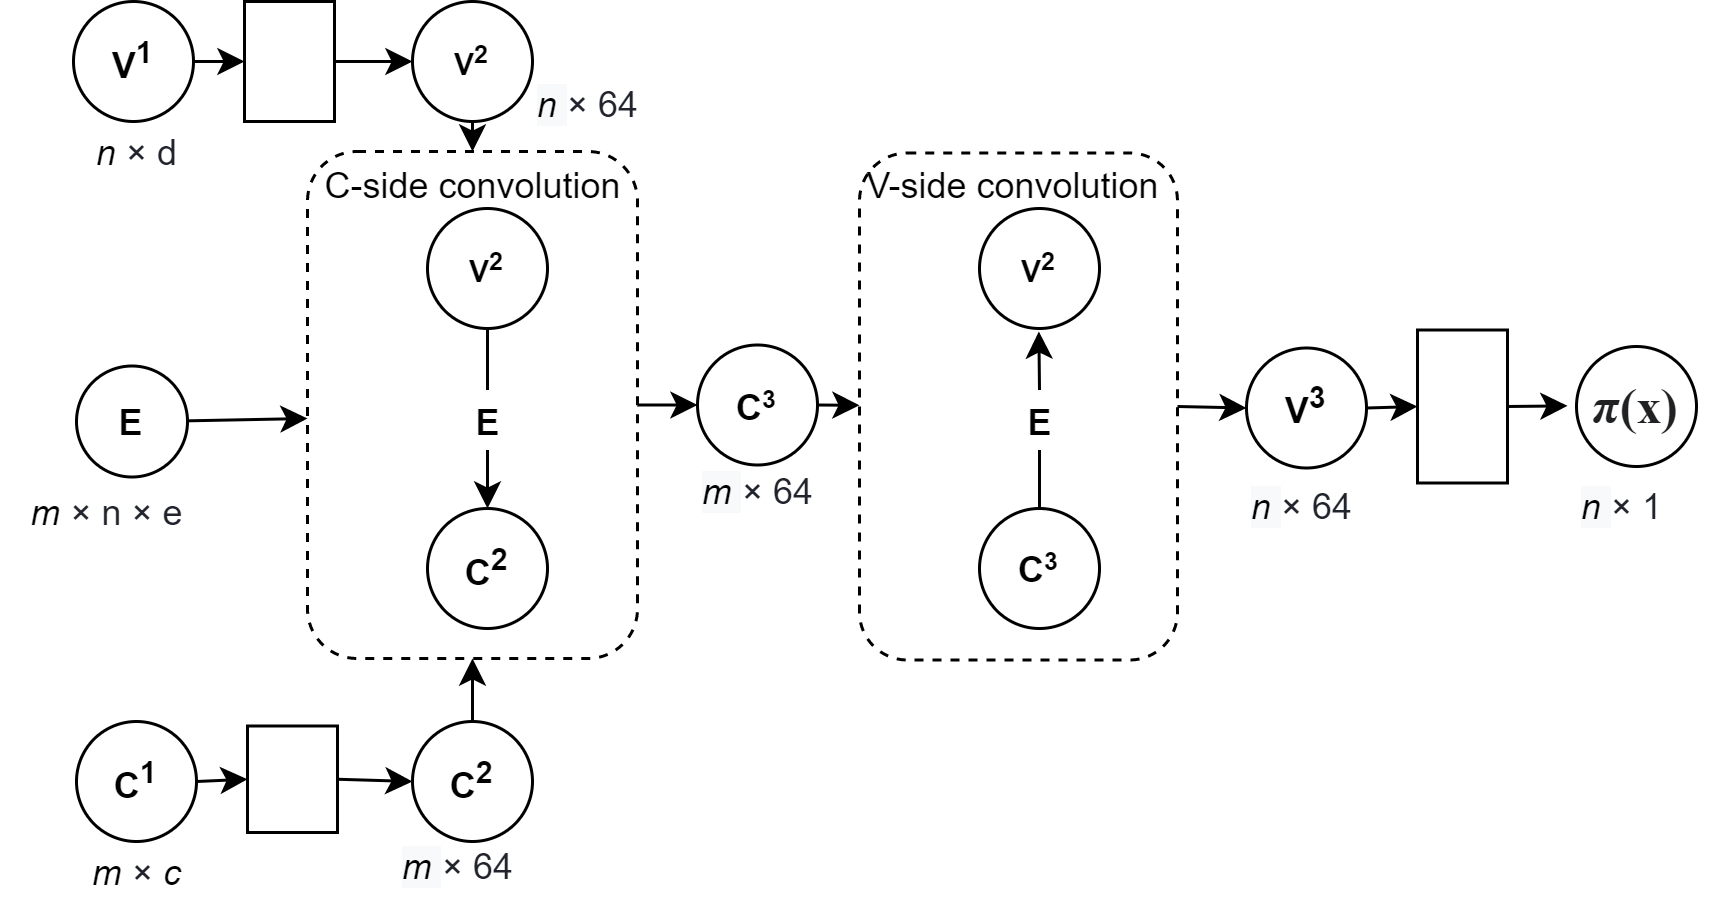
\includegraphics[width=\linewidth]{img/gnn_2.png}
    \caption{The Graph Convolutional Neural Network as specified in Gasse et al. (2019) \cite{gasse2019exact}.}
    \label{fig:gnn2}
\end{figure}






\subsection{Network Topologies}

As stated, the \gls{ML}-models used in the experiments are generated by iteratively ablating (removing components) from the original network. This results in models that are \gls{GCNN}s and models that are pure \gls{MLP}s, which will be compared for accuracy and efficiency on both \gls{GPU} and \gls{CPU}. 

The ablated models are chosen based on three basic assumptions that are assumed to be true based on the vast literature in deep learning\footnote{These assumptions are separate from the three research questions presented in \Cref{sec:int_questions}, and will not be covered in the same detail.} \cite{goodfellow2016deep}. The assumptions are stated as: 


\begin{enumerate}[label=(\roman*)]
    \item  It is assumed that increasing the capacity of the network correlates to increasing the number of computations \cite{goodfellow2016deep}. 
    \item  It is assumed that the variation in complexity will lead to differences in both accuracy and forward pass computation time \cite{goodfellow2016deep}. 
    \item  It is  assumed that the addition of the graph convolution will be a significant factor in the accuracy and efficiency of the models, particularly on the \gls{CPU}, based on the results in the appendix of Gupta et al. (2020) \cite{gupta2020hybrid}.
\end{enumerate}

Considering this, the experiments will be performed with a total of five models, meaning the original model and four models stemming from the iterative ablation of this model. Of these, two models will contain the graph convolution operation, and three will be Multi-layer Perceptrons that only use the variable data. 

Results in the specialization project this thesis is based on showed consistent and significant changes in the accuracy-efficiency trade-off were found with a similar selection of \gls{MLP} models, although these models relied on the extended variable feature set developed in Khalil et al. (2016) \cite{khalil2016learning}.

\textit{GNN2}, illustrated in \Cref{fig:gnn1}, is identical (except for the minor, commented details), to the original Gasse \gls{GCNN}.  

\textit{GNN1}, illustrated in \Cref{fig:gnn1}, is the model resulting from the first iteration of the ablation, which has reduced the number of layers in the embeddings and the output module. The graph convolutions are therefore unchanged.

\begin{figure}
    \centering
    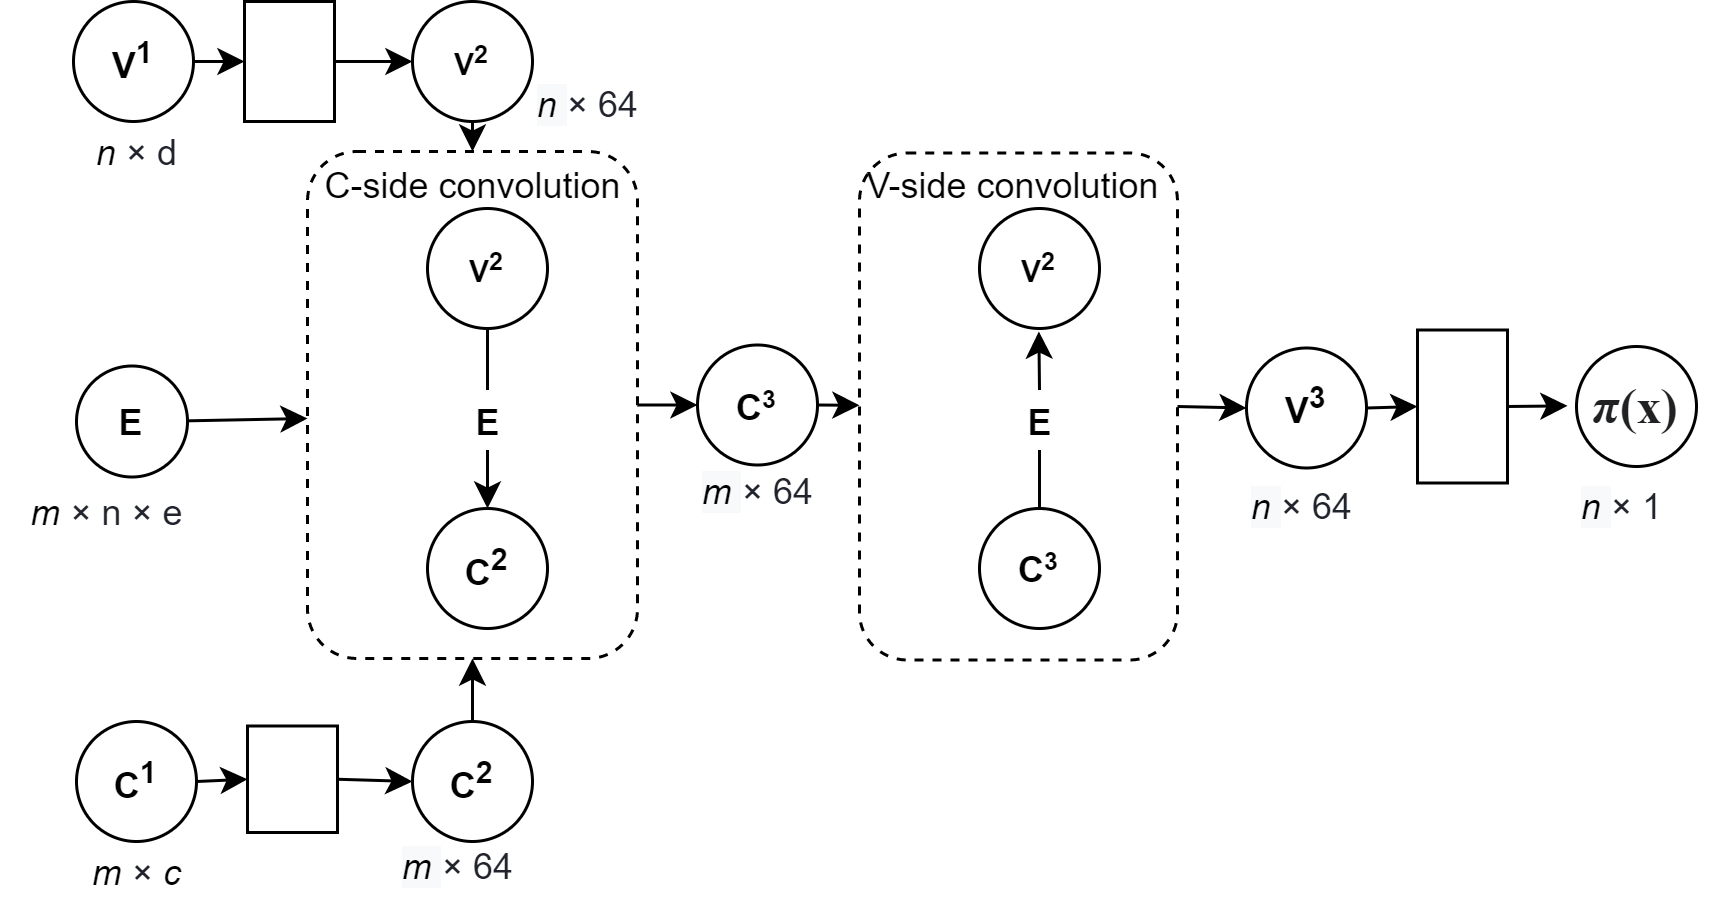
\includegraphics[width=\linewidth]{img/gnn_1.png}
    \caption{Topology of the ablated model GNN1.}
    \label{fig:gnn1}
\end{figure}

\textit{\gls{MLP}3} is illustrated in \Cref{fig:topo_mlp3}. The second ablation removes the convolutions in their entirety, resulting in an \gls{MLP} model consisting of the prenorm layer and embedding of the variable features with the output module. This equates to a four-layer \gls{MLP}


\textit{\gls{MLP}2} is illustrated in \Cref{fig:topo_mlp1}. The third ablation removes layers from the MLP3 model, yielding a network with lower capacity but fewer operations needed for evaluation. The two-layer \gls{MLP} also results in a minimal network for representing non-linear relations between the features and the scores. 


\textit{\gls{MLP}1} is illustrated in \Cref{fig:topo_mlp2}. The fourth ablation removes all hidden layers, resulting in an \gls{MLP} model consisting of the prenorm layer and embedding of the variable features with the output module. This is equivalent to finding the optimal linear combination of input parameters\footnote{To be exact, MLP1 is not a Multi-Layer Perceptron, however, the name is chosen to be consistent with the other models. The central difference between the models is whether they contain graph convolutions or not (given by the acronym) and the number of parameters (given by the number).}. A forward pass is equivalent to a single matrix multiplication. 


\begin{figure}
    \centering
    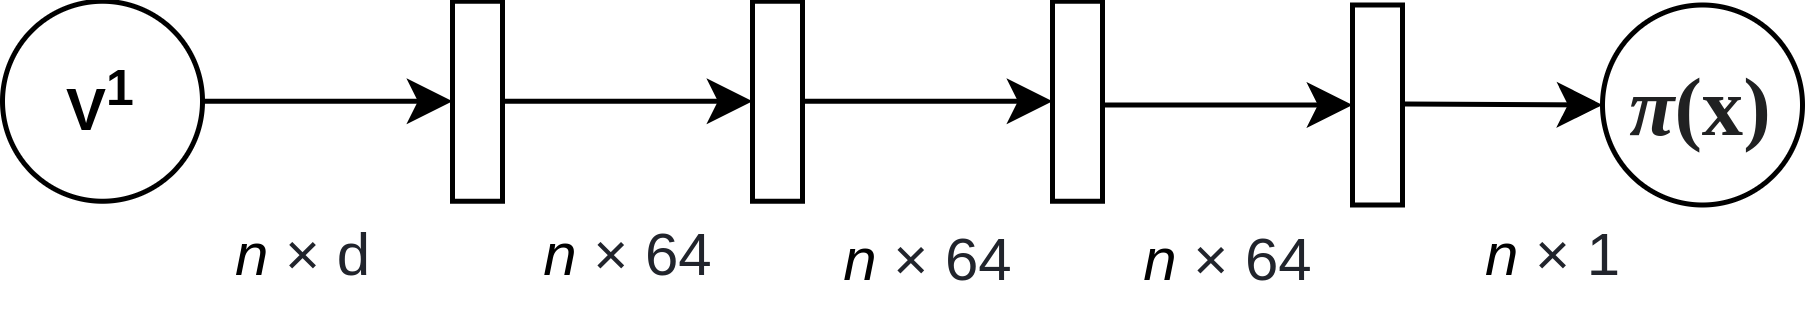
\includegraphics[width=0.8\linewidth]{img/mlp3.png}
    \caption{Topology of the larger sized MLP3 feed-forward network.}
    \label{fig:topo_mlp3}
\end{figure}

\begin{figure}
    \centering
    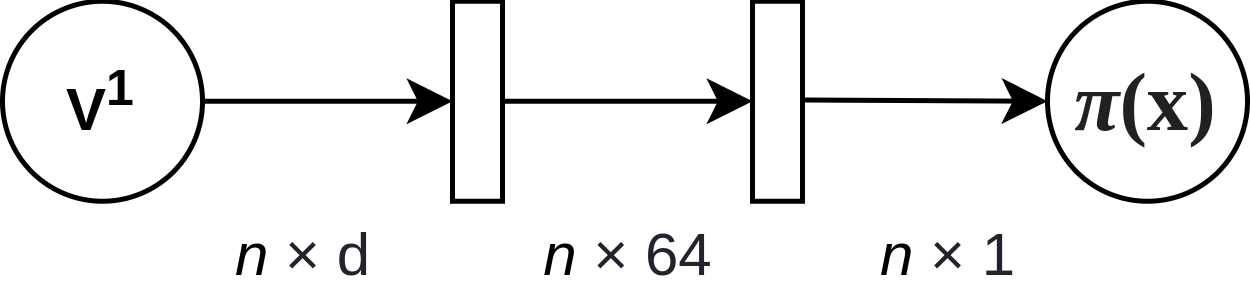
\includegraphics[width=0.55\linewidth]{img/mlp2.png}
    \caption{Topology of the medium sized MLP2 feed-forward network.}
    \label{fig:topo_mlp2}
\end{figure}

\begin{figure}
    \centering
    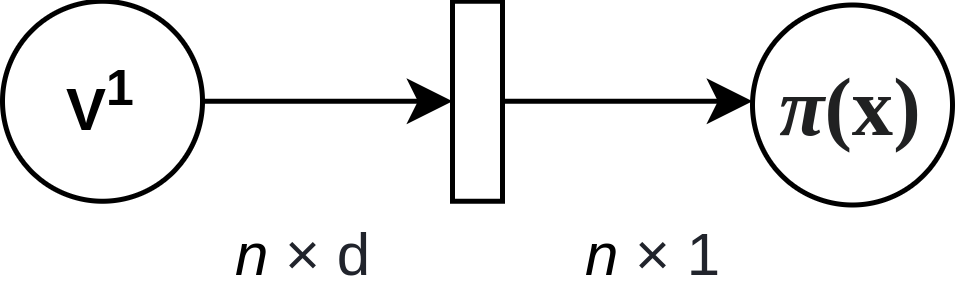
\includegraphics[width=0.45\linewidth]{img/mlp1.png}
    \caption{Topology of the smaller sized MLP1 feed-forward network.}
    \label{fig:topo_mlp1}
\end{figure}



\subsection{Network hyperparameters}

All hyperparameters except for the amount and size of the hidden layers is consistent for all models, in order to make a fairer judgment of the accuracy/efficiency trade-off. The activation function is the \textit{Recti-Linear Unit} (ReLU), expressed as $y = \max \{ 0, x\}$. This non-linear activation function is the least computationally expensive of the common activation functions. This is consistent with Gasse et al. (2019) \cite{gasse2019exact} and Gupta et al. (2020) \cite{gupta2020hybrid}.


\section{Training Protocol}\label{sec:trainingprotocol}

In this section, the training protocol is presented, which explains how the parameters of the models are learned.


\subsection{Loss function}

The problem is expressed as a two-class classification problem, where the classes are \textit{optimal variable} and \textit{sub-optimal variable}, respectively. The first class contains only the top variable from the strong branching evaluation. The loss function in binary classification is typically chosen as the binary cross-entropy loss function \cite{goodfellow2016deep}, calculated as:
\begin{align}
    \bm{\mathcal{L}}(\bm{\theta}) &= - \frac{1}{|\mathcal{D}|}\sum_{(\bm{x}, y) \in \mathcal{D}} \left( y_i \cdot \log( \hat y_i) + (1-y_i) \cdot \log(1 - \hat y_i) \right),
\end{align}
where $\mathcal{D}$ is the data set, $\hat y_i$ is the predicted class based on the sample features $x$, and $y_i$ is the classification by the Strong Branching expert.  
This means that for each branching decision, $n$ candidate variables will be given a score analogous to the probability of that variable being the best variable according to the strong branching expert policy. 

\subsection{Training method}

The parameters of the \gls{MLP} are trained via mini-batch gradient descent \cite{goodfellow2016deep}, and is performed using 
 the Adam optimizer \cite{kingma2017adam}. The Adam optimizer performs gradient descent with adaptive moments in both the first and second order \cite{kingma2017adam}. 
 The batch size (number of problems processed at once) is set to 32. The learning rate is reduced upon plateaus\footnote{\textit{Plateaus} are multiple epochs without reduction in the target loss.} in validation loss 
 by multiplying with $ 0.2 $. This is a well-known method to ensure convergence to a reasonably good local minimum \cite{goodfellow2016deep}.
 
 Further, the training has implemented an \textit{early stopping scheme}, to ensure that the models have converged, regardless of model complexity. If the validation loss does not decrease 16 epochs in a row, the model that resulted in the lowest validation loss is saved and the training process is stopped. This is because it is considered unlikely for the optimizer to improve the model after that amount of epochs without improvement. 
 
 All of these methods are implemented in order to give the fairest evaluation of the models, as individual hyperparameter optimization for each model would be too time-consuming to be performed. 


\subsection{Computer Hardware}

Training of the \gls{MLP}s is performed on an NVIDIA RTX2070 SUPER GPU (8GB VRAM). The \gls{BnB} solution efficiency evaluations are performed with an Intel i5-2500K \gls{CPU} (4 cores, 6 threads) running at 3.31 GHz. This is less expensive hardware compared to Gasse et al. (2019) \cite{gasse2019exact} and Gupta et al. (2020) \cite{gupta2020hybrid}, particularly the CPU. Variation in processing power is assumed to have an insignificant effect on the relative solution times of the methods, however, \gls{CPU}s with internal acceleration methods for matrix operations might give varying results \cite{vanhoucke2011improving}. It is assumed that the results on the chosen hardware yield a more pessimistic performance overall for the \gls{ML} based methods, and will therefore not be given too much attention in the thesis. Analysis of these differences in hardware and processing performance for both the classical and learned methods on both \gls{CPU} and \gls{GPU} is of interest, but far beyond the scope of this thesis. 



\section{Comparison Method}

The method in which the learned models are compared to each other and the classical branching policies is presented in this section.


\subsection{Classical Branching Policies}

The accuracy and efficiency of the algorithm with the learned branching policy are evaluated against three branching policies native to the \gls{SCIP} optimization suite, and explained in  more detail in \Cref{ssec:branchingpolicy}. 

First is the Full Strong Branching (\gls{FSB}) policy \cite{applegate1995finding}, the slow but accurate expert policy that performs Strong Branching at every node for every variable. This algorithm is not commonly used because of the computationally heavy variable decision process \cite{achterberg2004branching}.

Pseudo-cost Branching (\gls{PC}) is the fast but inaccurate branching policy \cite{gamrath2018measuring} that chooses the variable that maximizes the lower bound improvement according to the results of previous branching decisions \cite{benchiou1971experiments}.% This method does not compute anything for the candidate variables and relies only on previous results. 

Reliability Pseudo-cost Branching (\gls{RPC}) \cite{achterberg2004branching} combines \gls{FSB} and \gls{PC} by performing \gls{SB} on variables with low confidence in the pseudo-costs \cite{gamrath2018measuring}. \gls{RPC} is the default branching policy in the \gls{SCIP} \gls{BnB} solver. 

The classical variable selection policies will be implemented by configuring the priority of the branching policies in \gls{SCIP}. 


\subsection{Benchmarking}\label{ssec:benchmarking}

The learned branching policies are evaluated for both \textit{accuracy} and \textit{efficiency}. 

The accuracy of the policies is evaluated against the expert decisions of the Full Strong Branching Algorithm. This is done by evaluating the average \textit{top-k accuracy} over an unseen test set. Top-k accuracy measures whether the chosen branching variable was within the top k choices of the Strong Branching algorithm, based on the score given to each candidate variable by the algorithm. Only the learned models are measured in this regard. 

The efficiency of the policies is evaluated by exchanging the branching policy of the optimization solver and testing on the data set, as described in \Cref{sec:dataset}. The counting of nodes and time is done with the built in capabilities of \gls{Ecole}. %For the largest problems, solution time is limited to $ 45 $ minutes, and the number of problems the algorithm does not solve will be reported.
%The execution time is compared using python's \verb|time.proc_time()| function, which returns the \gls{CPU} process time \cite{rossum2009python}. 

The number of nodes processed by the algorithm will also be reported. Fewer nodes are not necessarily indicative of a better algorithm, however, this will be an important comparison, as it gives a proxy measurement of the accuracy/efficiency trade-off for the algorithms. 





\section{Software}

A number of comprehensive software libraries are required to perform the experiments in this thesis, this section presents the three most essential.  


\subsection{SCIP}

\textit{Solving Constraint Integer Programs }(\gls{SCIP})
\cite{achterberg2009scip}, is the \gls{CO} solver that lays the foundation for the data generation and model evaluation for the methods. It is considered the fastest non-commercial solver for \gls{MIP} and \gls{MINLP} problems \cite{gamrath2020scip}. It is written in C with wrappers for C++. The software is maintained by the\textit{ Zuse Institute Berlin} (ZIB) group. 

The \textit{SCIP Optimization Suite} contains, as of version 7, the simplex-based linear programming solver SoPlex \cite{wunderling1996soplex}, the automated decomposition solver GCG \cite{gamrath2010gcg}, the parallelization framework UG \cite{shinano2018ug} and the \gls{MILP} pre solving library PaPILO \cite{gamrath2020scip}.

In the experiments in this thesis, the LP solver and node selection algorithms are the most relevant, as most of the more complex capabilities of \gls{SCIP} are deactivated in order to make the results as fair and reproducible as possible. 





\subsection{PyTorch}

\textit{PyTorch} is the Python library that the machine learning models are written in. The library provides, most notably, dynamic eager execution, automatic differentiation, and \gls{GPU} acceleration \cite{paszke2019pytorch}. 

Necessary for constructing and training the graph convolutional neural networks, the \textit{PyTorch Geometric} library was used \cite{fey2019pytorchgeometric}. The library facilitates deep learning on data with irregular structures, such as graphs. This includes methods for sparse data GPU acceleration and efficient mini-batch handling \cite{fey2019pytorchgeometric}. 




\subsection{Ecole}\label{ssec:ecole}

To facilitate and standardize the development of \gls{ML}-based improvements of \gls{CO} algorithms, \textit{Extensible Combinatorial Optimization Learning Environments} (\gls{Ecole}) was developed \cite{prouvost2020ecole}, with the first version published in the last quarter of 2020. \gls{Ecole} aims to mimic the \textit{openAI Gym} framework \cite{brockman2016openai}, a popular framework for developing \gls{RL} models. It is a python library written largely in efficient C++. 
The library is based on the open-source solver \gls{SCIP} \cite{achterberg2009scip}.


It also provides \gls{CO} problem \textit{generators} for the four problem classes presented in this thesis. As of version 0.5, these generators are not completely correct, and in the problem generators from Gupta et al. (2020) \cite{gupta2020hybrid} were therefore used. These problems appear to be resolved in version 0.6.  


The theoretical basis for \gls{Ecole} is the \gls{PO-MDP} formulation for \gls{Ecole}, given in \Cref{sec:back_mdp}.
%The relevant functions and their \gls{PO-MDP} counterparts can be presented as follows \cite{prouvost2020ecole}:
%\begin{align*}
%    RewardFunction &\equiv \mathcal{R}\\
%ObservationFunction &\equiv \mathcal{O}\\
%reset\_dynamics() &\equiv p_\textit{init}(s_0)\\
%step\_dynamics() &\equiv p_\textit{trans}(s_{t+1}|s_t,a_t)\\
%reset() &\equiv s_0 \sim p_\textit{init}(s_0), r_0=R(s_0), o_0=O(s_0)\\ 
%step() &\equiv s_{t+1} \sim p_\textit{trans}(s_{t+1}|a_t,s_t)\\ r_t&=R(s_t)\\ o_t&=O(s_t)
%\end{align*}





\subsection{Development Environment}

The project is run on only open-source software, in order to support and further develop the commonly available tools for machine learning and mathematical programming. For reproducibility, the libraries and their respective versions are listed here, as well as in the publicly available code repository. 

The project code is written in 
\verb|python 3.8.5| \cite{rossum2009python}, and uses               
\verb|pytorch 1.6.0| \cite{paszke2019pytorch} for the machine learning models.           

For \gls{GPU} accelerated training, 
\verb|cudnn 7.6.5| and 
\verb|cudatoolkit 10.2.89| \cite{kirk2008nvidia} is used. 

The optimization problems are solved using the \verb|SCIP 7.0.2| Optimization Suite \cite{gamrath2020scip}, using the 
\verb|SoPlex 4.0.1| \cite{wunderling1996soplex} linear programming solver to solve the relaxed problems. The Python interface
\verb|PySCIPOpt 3.0.4| \cite{maher2016pyscipopt} is used in and alongside \gls{Ecole} to facilitate communication with \gls{SCIP}.

The computer is running the \verb|Ubuntu 20.04.2| Linux distribution.


\subsection{Code Repository}

As stated, the code for reproducing the experiments is given in a publicly available code repository, found at \url{https://github.com/Sandbergo/branch2learn}. It is intended to be similar to the source code for Gasse et al. (2019) \cite{gasse2019exact}, and to be extensible in order to facilitate further work. 

A presentation of the code is given in \verb|README.md|, with installation instructions in \verb|INSTALLATION.md|. Installation requires some manual installation but is mostly done using \verb|Anaconda|. The eponymous subdirectory \verb|branch2learn| contains python scripts for running the respective processes of training and evaluating the models: \verb|00_generate_instances.py|, \verb|01_generate_data.py|, \verb|02_train.py|,
\verb|03_test.py|, \\
\verb|04_evaluate.py|, and \verb|05_evaluate_standard.py|. In addition, the directories for the models and utility functions are found there.

The directory \verb|scripts| contains bash-scripts for reproducing all experiments used in this thesis. 
\chapter{Results}\label{cha:results}

In this chapter, the results of the experiments are reported, as described in \Cref{cha:methods}. Several sections share formulations with sections from the corresponding chapter in the project report \textit{Multi-layer Perceptrons for Branching in Mixed-Integer Linear Programming} (2020). 


\section{Dataset Generation}\label{sec:datagen}

Problem instances are generated as described in \Cref{ssec:probleminstances}. In total, $2000$ training instances, $500$ validation instances and $ 500 $ test instances are created. These are of size $100 \times 500$ for the combinatorial auction problems and $100 \times 500$ for the set covering problems, as stated in \Cref{sec:dataset}. This information is shown in \Cref{tab:instances}.

The generated problem instances are then solved as specified in \Cref{ssec:expertsolutiongeneration}. This results in a total of 50000 training samples, 10000 validation samples and 10000 test samples for the combinatorial auctions problems, and the same for the set covering problems. This is also shown in \Cref{tab:instances}

AVERAGE NUMBER OF CONSTRAINTS

$250$ problem instances are generated for evaluating the efficiency of the models. In addition, as is done in \cite{gasse2019exact}, additional larger problems are generated in order to evaluate the models' ability to perform on more difficult problems. This includes $50$ medium-sized instances and $20$ large-sized instances. These problems are shown in \Cref{tab:samp_transf}.

\begin{scriptsize}
\begin{table}[ht]
	\centering
	\begin{tabular}{llccc}
		\toprule
		  && \multicolumn{1}{c}{Train} & \multicolumn{1}{c}{Validate} & \multicolumn{1}{c}{Test}\\
		  \cmidrule(lr){3-3} \cmidrule(lr){4-4} \cmidrule(lr){5-5}
		  \multirow{3}{*}{Auctions} & Dimensions & $100 \times 500$ & $100 \times 500$ & $100 \times 500$ \\
		% \midrule
		& Instances & 2000 &  500  & 250\\
		& Samples & 50000 &  10000  & 10000 \\
		\addlinespace
		\multirow{3}{*}{Setcover} & Dimensions & $500\times1000$ & $500\times1000$ & $500\times1000$\\
		% \midrule
		 & Instances & 2000 &  500  & 500 \\
		 & Samples & 50000 &  10000  & 50000 \\
		% \addlinespace
		\bottomrule
	\end{tabular}
	\caption{Data set, dimensions and number of problem instances for each problem class.}\label{tab:instances}
\end{table}
\end{scriptsize}

\begin{scriptsize}
\begin{table}[ht]
	\centering
	\begin{tabular}{llccc}
		\toprule
		&& \multicolumn{1}{c}{Small} & \multicolumn{1}{c}{Medium} & \multicolumn{1}{c}{Large}\\
		  \cmidrule(lr){3-3} \cmidrule(lr){4-4} \cmidrule(lr){5-5}
		  \multirow{2}{*}{Auctions} & Dimensions & $100 \times 500$ & $200 \times 1000$ & $300 \times 1500$ \\
		% \midrule
		& Instances & 250 &  50  & 20\\
		\addlinespace
		\multirow{2}{*}{Setcover} & Dimensions & $500\times1000$ & $1000\times1000$ & $2000\times1000$\\
		% \midrule
		 & Instances & 250 &  50  & 20 \\
		% \addlinespace
		\bottomrule
	\end{tabular}
	\caption{Data set, dimensions and number of problem instances for each problem class.}\label{tab:samp_transf}
\end{table}
\end{scriptsize}




\section{Training}\label{sec:res_training}

The training was performed as described in \Cref{sec:trainingprotocol}. 
The training graph for MLP2 on the combinatorial auction data set is shown in \Cref{fig:training_mlp2}, and the training graph for GNN1 on the setcover data set is shown in \Cref{fig:training_gnn1}. The Training and validation loss quickly converges before flattening out. There is no discernible difference between training and validation loss. Loss graphs for the other models are not presented, as they are very similar, and are therefore considered to be of little interest. 
%
\begin{figure}[h]
    \centering
    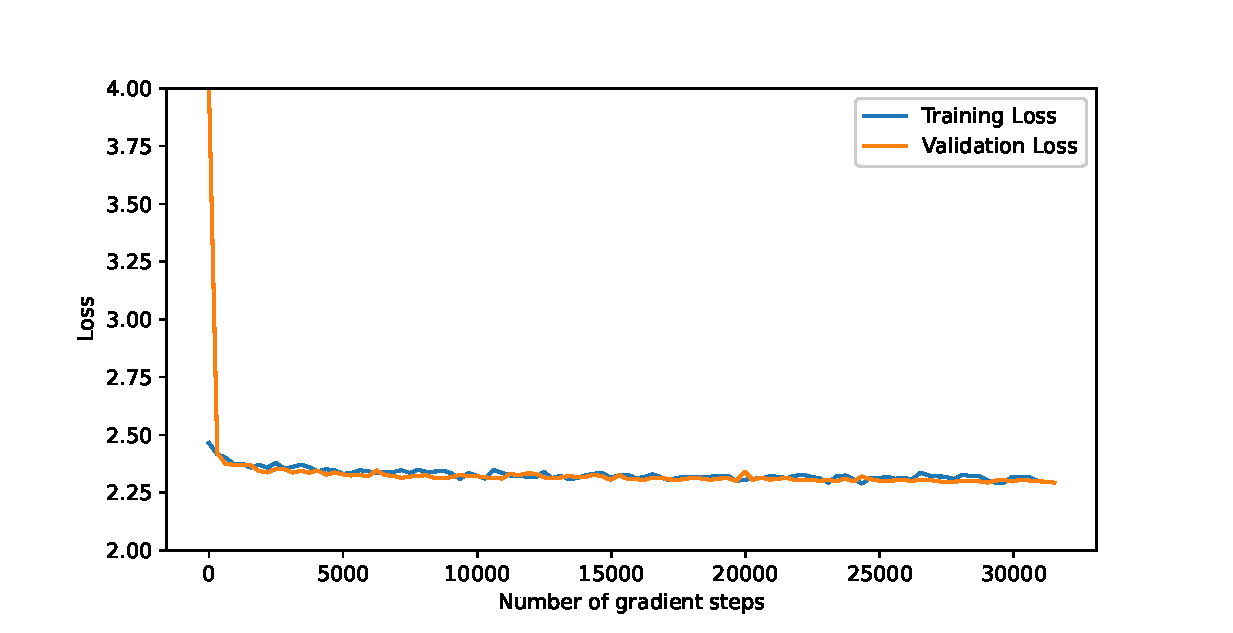
\includegraphics[width=\textwidth]{img/loss70.eps}
    \caption{Training graph for MLP2 on the combinatorial auctions data set.}
    \label{fig:training_mlp2}
\end{figure}

\begin{figure}[h]
    \centering
    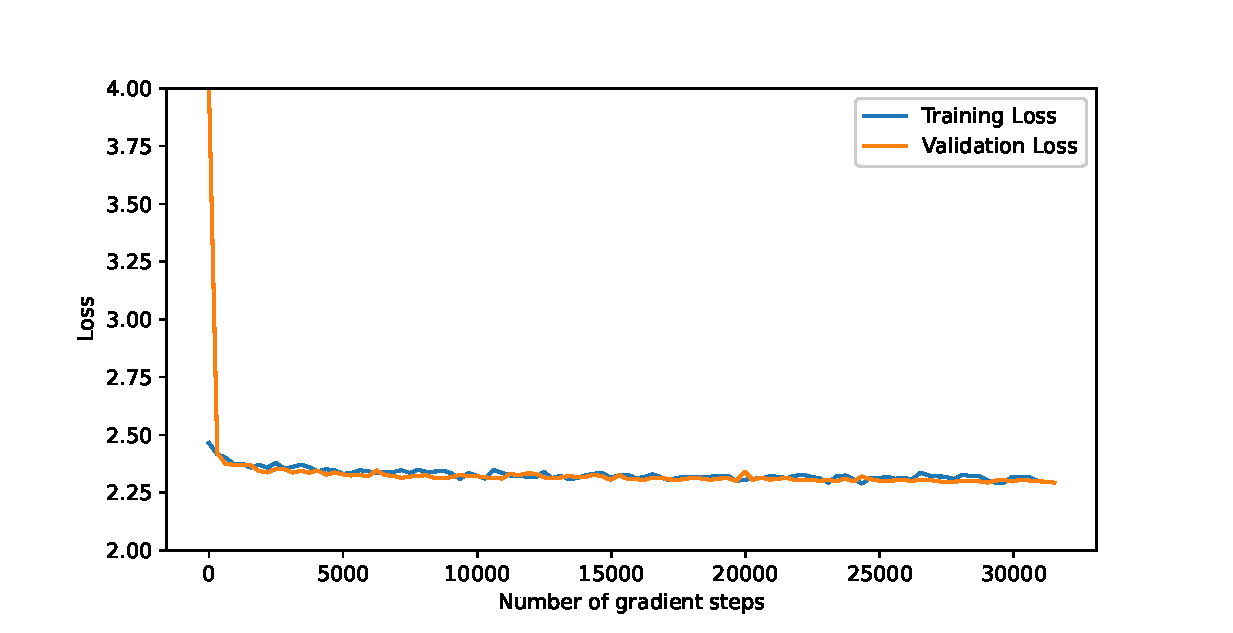
\includegraphics[width=\textwidth]{img/loss70.eps}
    \caption{Training graph for GNN1 on the set covering data set.}
    \label{fig:training_gnn1}
\end{figure}



\section{Accuracy}\label{accuracy}\label{sec:res_accuracy}


\begin{scriptsize}
\begin{table}[ht]
	\centering
	\begin{tabular}{lrrrrrrr}
		\toprule
		& \multicolumn{3}{c}{Combinatorial Auction} & \multicolumn{3}{c}{Set Covering}\\ 
		\cmidrule(lr){2-4} \cmidrule(lr){5-7}
		Model & acc@1 & acc@5 & acc@10 & acc@1 & acc@5 & acc@10 \\
		\midrule
		random & 0.0 \% & 0.0 \% & 0.0 \% & 0.0 \% & 0.0 \% & 0.0 \%\\
		MLP1 & 30.3 \% & 62.8 \% & 79.4 \% & 0.0 \% & 0.0 \% & 0.0 \%\\
		MLP2 & 50.1 \% & 78.9 \% & 89.9 \% & 46.0 \% & 74.2 \% & 87.2 \%\\
		MLP3 & 50.2 \% & 79.3 \% & 90.1 \% & 46.2 \% & 74.7 \% & 87.4 \%\\
		GNN1 & 53.0 \% & 87.5 \% & 95.9 \% & 56.9 \% & 88.6 \% & 96.8 \%\\
		GNN2 & 53.0 \% & 87.1 \% & 96.0 \% & 56.8 \% & 88.5 \% & 96.9 \%\\
		\addlinespace
		\bottomrule
	\end{tabular}
	\caption{Top-k accuracy scores for combinatorial auctions and set covering on the test set.}\label{tab:accs}
\end{table}
\end{scriptsize}

% CAUCTIONS
% MLP1 0.30329361 0.43040384 0.5133234  0.57414763 0.62793777 0.66972857
%0.70506455 0.7397385  0.76903343 0.79443893
%[0.50099305 0.61717974 0.69298246 0.7469381  0.78930818 0.82000993
%0.84640847 0.86701423 0.88339954 0.89920556]
% 0.50281364 0.61924859 0.69546508 0.75       0.79319762 0.82116849
% 0.84789805 0.8683383  0.8857994  0.90143992]
% [0.52962595 0.68884475 0.7744952  0.8326713  0.87520689 0.90292949
% 0.92303873 0.938762   0.95076134 0.95945051]
% [0.52962595 0.68636213 0.7744952  0.83325058 0.87065541 0.90052963
% 0.92171466 0.93776895 0.95092685 0.96027805]
 
% SETCOVER
% MLP1 [20.4 30.2 36.8 41.8 45.7 48.8 51.8 54.5 56.6 58.5] %
% MLP2 [0.4604 0.5681 0.6453 0.7026 0.7424 0.7804 0.8085 0.8315 0.853  0.8719]
% MLP3 [0.4616 0.5721 0.652  0.7054 0.7472 0.7834 0.8127 0.8363 0.8568 0.8744]
% GNN1 [0.5693 0.7178 0.7961 0.8507 0.8862 0.9108 0.9317 0.9486 0.9584 0.9682]
% GNN2 [0.5679 0.7139 0.7955 0.8477 0.8848 0.9101 0.9336 0.9496 0.961  0.9688]
The accuracy of the models are measured by the top-k accuracy, as specified in \cref{ssec:benchmarking}.
The top-k accuracy scores for k equal to 1, 5 and 10 for the models along with the benchmark accuracy for random variable selection is shown in \Cref{tab:accs}. Top-k accuracy for this application is defined as the number of selected branching variables within the top k variables as determined by the Strong Branching evaluation. 
% https://scikit-learn.org/dev/modules/model_evaluation.html#top-k-accuracy-score

Comparison with the random variable selection policy shows considerable improvement in favor of the trained models. Accuracy decreases with the ablations, although there is little difference between GNN2 and GNN1, and MLP3 and MLP2, respectively. MLP1 performs considerably poorer than the other models, indicating that a non-linear relationship between the variable features and the variable score is beneficial. There is also a noteworthy decrease in accuracy after removing the graph convolutions, indicating that the module aids in prediction.

A comparison of the differences between models of the two problem classes shows that the decrease in accuracy from GNN1 to MLP3 is around three times larger for the setcovering problems. This indicates that the addition of different problem classes in the evaluation of branching policies is necessary.

Note that the GNN2 model should have similar accuracy to the corresponding model in Gasse et al. (2019) \cite{gasse2019exact}, however, the models have almost 10 \% lower accuracy. The cause for this is unknown, and the analysis of the models will not be affected by this. 

\begin{comment}
    
\begin{figure}
    \begin{tikzpicture}
      \begin{axis}[
        mlineplot,
        ylabel={Accuracy [\%]},
        xlabel={Top k},
        width=\textwidth,
        height=7cm,
	    ymin=0.0,   ymax=1.0,
	    xtick=data,
	    legend style={at={(0.01,0.9)},anchor=west}
      ]
        \addplot plot coordinates{(1, 0.413) (2, 0.538) (3, 0.621) (4, 0.681) (5, 0.732) (6, 0.770) (7, 0.800) (8, 0.827) (9, 0.849) (10, 0.867)};
        \addplot plot coordinates{(1, 0.437) (2, 0.568) (3, 0.653) (4, 0.717) (5, 0.767) (6, 0.805) (7, 0.835) (8, 0.860) (9, 0.881) (10, 0.899)};
        \addplot plot coordinates{(1, 0.435) (2, 0.568) (3, 0.652) (4, 0.716) (5, 0.765) (6, 0.802) (7, 0.831) (8, 0.858) (9, 0.879) (10, 0.897)};
        \addplot+ plot coordinates{(1, 0.019) (2, 0.034) (3, 0.047) (4, 0.060) (5, 0.071) (6, 0.081) (7, 0.090) (8, 0.098) (9, 0.107) (10, 0.115)};
        %\addplot+[samples=100] {sin(deg(2*x))};
        \legend{MLP1,MLP2,MLP3,Random}
        
      \end{axis}
    \end{tikzpicture}
    \caption{Top k accuracy of trained models and random variable selection on test set. MLP2 and MLP3 nearly indistinguishable.}
    \label{fig:topk}
\end{figure}
\end{comment}
% 0 0.0 acc@1: 43.7 acc@2: 56.8 acc@3: 65.4 acc@4: 71.7 acc@5: 76.6 acc@6: 80.3 acc@7: 83.3 acc@8: 85.9 acc@9: 88.0 acc@10: 89.9

% 61 acc@0:  0.0 acc@1: 41.3 acc@2: 53.8 acc@3: 62.1 acc@4: 68.1 acc@5: 73.2 acc@6: 77.0 acc@7: 80.0 acc@8: 82.7 acc@9: 84.9 acc@10: 86.7

% 70 acc@0:  0.0 acc@1: 43.5 acc@2: 56.8 acc@3: 65.2 acc@4: 71.6 acc@5: 76.5 acc@6: 80.2 acc@7: 83.1 acc@8: 85.8 acc@9: 87.9 acc@10: 89.7


\section{Efficiency}\label{sec:res_efficiency}

Eight branching strategies were compared on the problem data set of three different problem sizes. The branching strategies are Full Strong Branching, Reliability Pseudo-cost branching, and the five learned models. The results for the combinatorial auctions problems are shown in \Cref{tab:results1_cauction} and for the setcovering problems in \cref{tab:results1_set}. \textit{Time} is the mean solution time, \textit{nodes} is the mean number of nodes in the solution graphs (calculated in accordance with the findings of Gamrath et al. (2018) \cite{gamrath2018measuring}, \textit{time/node}) is the average time per node, calculated by dividing the two means, and \textit{parameters} is the number of (trainable) parameters of the model. TIME/CANDIDATES? In other works relating to node and time measurements when comparing branching policies, a variant of the shifted geometric mean is used. This is not done in this thesis, see \cref{sec:distributions} for a short discussion on this. 
The branching strategy with the shortest mean solution time is marked bold for the \gls{CPU} and \gls{GPU} times. 

The results show that the ablation from GNN2 to GNN1 does not reduce the time per node, neither does the removal of hidden layers between the models MLP3 and MLP2. Time per node is considerably reduced after the graph convolutions are removed and reduced again when the model's hidden layers are removed. This is consistent over both the \gls{GPU} and \gls{CPU} variants.  



\Cref{fig:cauctions_bar} and \Cref{fig:set_bar} shows the results for the results from \cref{tab:results1_cauction} and \cref{tab:results1_set}, respectively, including $95 \%$ confidence intervals calculated under the assumption that the solution times are normally distributed.

Note also that the time per node is not equal between the two problem classes --- the average number of candidate variables per node will vary between problems.  
% \usepackage{booktabs}
 
% MLP2 CUDA: nb nodes     550 +- 1013 |  time  13.37 +-  20.60 | 100
\begin{scriptsize}
\begin{table}[ht]
	\centering
	\begin{tabular}{lrrrrrrr}
	    \toprule
		Model & Time (s) & Nodes  & Time/node (ms) & parameters \\
		\midrule
		FSB & 0 & 0 & 0 & --- \\
		PC  & $1.96 \pm 0.84$ & $355 \pm 358$ & $5.5$ & ---\\
		RPC & $2.73 \pm 1.18$ & $16 \pm 30$ & $ 171.1$ & ---\\
		\addlinespace
		MLP1\textsubscript{g} & $1.84 \pm 0.83$ & $282 \pm 362$ & $6.5$  & 0\\
		MLP2\textsubscript{g} & $1.60 \pm 0.44$ & $123 \pm 116$ & $13.0$ & 0\\
		MLP3\textsubscript{g} & $1.62 \pm 0.45$ & $121 \pm 112$ & $13.4$ & 0\\
		GNN1\textsubscript{g} & $1.65 \pm 0.45$ & $97 \pm 85$   & $17.0$ & 0\\
		GNN2\textsubscript{g} & $1.63 \pm 0.44$ & $95 \pm 80$   & $17.2$ & 0\\
		\addlinespace
		MLP1\textsubscript{c} & $1.78 \pm 0.78$ & $280 \pm 394$ & $6.4$  & 0\\
		MLP2\textsubscript{c} & $3.12 \pm 1.28$ & $123 \pm 114$ & $25.4$ & 0\\
		MLP3\textsubscript{c} & $3.24 \pm 1.35$ & $120 \pm 112$ & $27.0$ & 0\\
		GNN1\textsubscript{c} & $5.06 \pm 2.80$ & $96 \pm 81$   & $52.7$ & 0\\
		GNN2\textsubscript{c} & $5.10 \pm 2.92$ & $97 \pm 81$   & $52.6$ & 0\\
		\bottomrule
	\end{tabular}
	\caption{Combinatorial auction solving efficiency.}\label{tab:results1_cauction}
\end{table}

\begin{table}[ht]
	\centering
	\begin{tabular}{lrrrrrrr}
		\toprule
		Model & Time (s) & Nodes  & Time/node (ms) & parameters \\
		\midrule
		FSB & $25.02 \pm  19.25$ & $77 \pm 64$ & $324.9$ & ---\\
		PC  & $7.78 \pm 9.50$ & $749 \pm 1634$ & $10.4$ & ---\\
		RPC & $10.68 \pm 8.01$ & $295 \pm 895$ & $36.2$ & ---\\
		\addlinespace
		MLP1\textsubscript{g} & $ 23.58 \pm  38.93$ &  $1321 \pm 2354$ &  $  17.8$& 20\\
		MLP2\textsubscript{g} & $15.26 \pm 22.30 $ &  $ 522 \pm  909 $ &  $  29.2$ & 1344\\
		MLP3\textsubscript{g} & $16.45 \pm 22.58$ & $515 \pm 808 $  & $31.9$ & 9702\\
		GNN1\textsubscript{g} & $11.63 \pm 16.66$ & $272 \pm 506 $  & $42.8$ & 52083\\
		GNN2\textsubscript{g} & $11.18 \pm 11.51$ & $264 \pm 357 $  & $42.3$ & 64562\\
		\addlinespace
		MLP1\textsubscript{c} & $23.85 \pm 34.68$ & $1303 \pm 2308$ & $17.7$ & 20\\
		MLP2\textsubscript{c} & $17.26 \pm 20.53$ & $521 \pm 887$   & $33.1$ & 1344\\
		MLP3\textsubscript{c} & $18.46 \pm 23.24$ & $523 \pm  908$  & $35.3$ & 9702\\
		GNN1\textsubscript{c} & $68.59 \pm 97.11$ & $308 \pm 460$   & $222.6$ & 52083\\
		GNN2\textsubscript{c} & $72.37 \pm 112.80$ & $324 \pm 523$  & $223.4$ & 64562\\
		\bottomrule
	\end{tabular}
	\caption{Setcover solving efficiency.}\label{tab:results1_set}
\end{table}
\end{scriptsize}
%[05-10 21:02:43.02] Model:   mlp1
%[05-10 21:02:43.02] Device:  cpu
%[05-10 21:02:43.03] ------ setcover, small ------
%[05-10 21:47:49.72]  nb nodes    1303 +- 2308 |  time  23.85 +-  34.68 | completed   250
%[05-10 21:47:49.72] End of evaluation.
%(ecole) �� ~/git/branch2learn python branch2learn/04_evaluate.py -m mlp1 -g 0
%[05-10 22:42:42.31] Model:   mlp1
%[05-10 22:42:42.31] Device:  cuda
%[05-10 22:42:42.33] ------ setcover, small ------
%[05-10 23:27:49.03]  nb nodes    1322 +- 2346 |  time  20.62 +-  33.04 | completed   250
% 04-27 20:24:04.15] Policy:   fsb
%[04-27 22:08:43.84]  nb nodes      77 +-   64 |  time  25.02 +-  19.25 | completed   250
\begin{figure}[ht]
    \centering
    \begin{tikzpicture}
    \begin{axis}[
        width=\linewidth,
        axis x line*=bottom,
        axis y line*=left,
    	ylabel={Solution time [s]},
    	xlabel={Branching policy/model},
    	ymajorgrids=true,
    	ybar=5pt,% configures `bar shift'
    	bar width=9pt,
        xticklabels={PC,RPC,MLP1,MLP2,MLP3,%
		GNN1,GNN2},
		xtick=data,
		%enlarge x limits=0.15,
        %enlarge y limits=0.05,
        %restrict y to domain=0:6
        ymin=0.0,   ymax=6.0,
	    legend style={at={(0.01,0.9)},anchor=west,legend columns=-1}
    ]
    \addplot[color=black,fill=black!35,error bars/.cd,y dir=both,y explicit,]
    coordinates{
       (1,1.96) +-(0.0,0.1043)
       (2,2.73) +-(0.0,0.146)
       (3,1.78) +-(0.0,0.0967)
       (4,3.12) +-(0.0,0.159)
       (5,3.24) +-(0.0,0.167)
       (6,5.06) +-(0.0,0.347)
       (7,5.10) +-(0.0,0.362)
    };
    %negativ
    \addplot[color=black,fill=black!10,error bars/.cd,y dir=both,y explicit,]
    coordinates {
      %(1,0.9365) +- (0.00587,0.00587)
      %(2,0.1435) +- (0.01737,0.01737)
      (3,1.84) +-(0.0,0.103)
      (4,1.60) +-(0.0,0.0545)
      (5,1.62) +-(0.0,0.0558)
      (6,1.65) +-(0.0, 0.0558)
      (7,1.63) +-(0.0, 0.0558)
};
    \legend{CPU,GPU}
    \end{axis}
    \end{tikzpicture}
    \caption{Combinatorial Auction small problem mean solution time GPU and CPU.}
    \label{fig:cauctions_bar}
\end{figure}

\begin{figure}[ht]
    \centering
    \begin{tikzpicture}
    \begin{axis}[
        width=\linewidth,
        axis x line*=bottom,
        axis y line*=left,
    	ylabel={Solution time [s]},
    	xlabel={Branching policy/model},
    	ymajorgrids=true,
    	ybar=5pt,% configures `bar shift'
    	bar width=9pt,
        xticklabels={PC,RPC,MLP1,MLP2,MLP3,%
		GNN1,GNN2},
		xtick=data,
		%enlarge x limits=0.15,
        %enlarge y limits=0.05,
        %restrict y to domain=0:6
        ymin=0.0,   ymax=90.0,
	    legend style={at={(0.01,0.9)},anchor=west,legend columns=-1}
    ]
    \addplot[color=black,fill=black!35,error bars/.cd,y dir=both,y explicit,]
    coordinates{
       (1,7.78) +-(0.0, 1.18)
       (2,10.68) +-(0.0,0.993)
       (3,39.70) +-(0.0, 6.83)
       (4,17.26) +- (0.0, 2.6)
       (5,18.46) +- (0.0, 2.9)
       (6,68.59) +-(0.0,12)
       (7,72.37) +-(0.0,14)
    };
    %negativ
    \addplot[color=black,fill=black!10,error bars/.cd,y dir=both,y explicit,]
    coordinates {
      %(1,0.9365) +- (0.00587,0.00587)
      %(2,0.1435) +- (0.01737,0.01737)
      (3,23.58) +- (0.0, 4.86)
      (4,15.26) +- (0.0, 2.8)
      (5,16.45) +-(0.0,2.8)
      (6,11.63) +-(0.0, 2.07)
      (7,11.18) +-(0.0, 1.43)
};
    \legend{CPU,GPU}
    \end{axis}
    \end{tikzpicture}
    \caption{Set covering small problem mean solution time GPU and CPU.}
    \label{fig:set_bar}
\end{figure}


\begin{comment}
    
\begin{figure}
    \centering
    \begin{tikzpicture}
    
      \def\MarkSize{.75em}
      \protected\def\ToWest#1{%
        \llap{#1\kern\MarkSize}\phantom{#1}%
      }
      \protected\def\ToSouth#1{%
        \sbox0{#1}%
        \smash{%
          \rlap{%
            \kern-.5\dimexpr\wd0 + \MarkSize\relax
            \lower\dimexpr.375em+\ht0\relax\copy0 %
          }%
        }%
        \hphantom{#1}%
      }
    \begin{axis}[ xlabel={CPU time}, ylabel={GPU time}, width=10cm, height=10cm, ymin=1.0, ymax=5.5, xmin=1.0,   xmax=5.5, ymajorgrids=true,
    xmajorgrids=true,]v
    \addplot[scatter,mark=*,only marks, point meta=x,nodes near coords*={\data},
    visualization depends on={value \thisrow{dataname} \as \data},] 
    table [x=x,y=y]{
    x       y       dataname
    1.84    1.78    MLP1
    1.60    3.12    \ToSouth{MLP2}
    1.62    3.24    MLP3
    1.65    5.06    \ToSouth{GNN1}
    1.63    5.10    GNN2
    };
    \end{axis}
    \end{tikzpicture}
    \caption{Combinatorial Auction small problem mean solution time GPU and CPU.}
    \label{fig:gpu_cpu}
\end{figure}
\end{comment}


In Gasse et al. (2019) \cite{gasse2019exact} and Gupta et al. (2020), the models are also evaluated by their performance on larger problem sizes, as a method of measuring the models' ability to generalize.
This is a time consuming process, and therefore only a select number of models is used: MLP1, MLP2 and GNN1, as these represent the variations that are shown in \cref{fig:cauctions_bar} and \cref{fig:set_bar}.

The result is shown in \cref{tab:results_trans_cauction}, where \textit{time} and \textit{nodes} is measured as in \cref{tab:results1_cauction} and \cref{tab:results1_set}.
\textit{completed} is the number of problems where optimality was achieved within the time limit of 45 minutes and is only applicable for the large problem size. 

GNN1 and MLP2 perform competitively on the \gls{GPU}, while the \gls{MLP} suffers from the consequences of poor variable branching choices, leading to a very poor performance. 

% including transfer learning 

\begin{scriptsize}
\begin{comment}\begin{table}[ht]
	\centering
	\begin{tabular}{lrrrrrrr}
		\toprule
		& \multicolumn{2}{c}{Small} & \multicolumn{2}{c}{Medium} & \multicolumn{3}{c}{Large}\\ \cmidrule(lr){2-3} \cmidrule(lr){4-5} \cmidrule(lr){6-8}
		Model & Time (s) & Nodes  & Time (s) & Nodes & Time (s) & Nodes & Completed\\
		\midrule
		FSB & 0 & 0 & 0 & 0 & 0 & 0 & 0 / 20\\
		PC  & $7.78 \pm 9.50$ & $749 \pm 1634$ & $107.89 \pm 222.90 $ & $11549 \pm 26613$ & $1931.49 \pm 891.79$ & $14133$ & 12 / 20\\
		RPC & 0 & 0 & $92.85 \pm 163.33$ & $7085 \pm 17136.63$ & $1583.41 \pm 953.98$ & $112234 \pm 68953$ & 14 / 20\\
		\addlinespace
		MLP1\textsubscript{g} & $36.89 \pm 57.71$ & $2232 \pm 3442$ & 0 & 0 & 0 & 0 & 0 / 20\\
		MLP2\textsubscript{g} & $16.24 \pm 27.27$ & $545 \pm 1120$ & 0 & 0 & 0 & 0 & 0 / 20\\
		GNN1\textsubscript{g} & $11.63 \pm 16.66$ & $272 \pm 506 $& 0 & 0 & 0 & 0 & 0 / 20\\
		\addlinespace
		MLP1\textsubscript{c} & $39.70 \pm 55.09$ & $2242 \pm 3486$ & 0 & 0 & 0 & 0 & 0 / 20\\
		MLP2\textsubscript{c} & $16.70 \pm 17.78$ & $513 \pm 720$ & $537.33 \pm 1289.62$ & $12546 \pm 30600$ & $7725.52 \pm 3109.38$ & $121066$ & 3 / 20\\
		GNN1\textsubscript{c} & $68.59 \pm 97.11$ & $308 \pm 460$ & $1697.88 \pm 2278.39$ & $4104 \pm 5208$ & --- & --- & 0 / 20\\
		\bottomrule
	\end{tabular}
	\caption{Setcover solving time on larger problem sets.}\label{tab:results_trans_set}
\end{table}\end{comment}
\begin{table}[ht]
	\centering
	\begin{tabular}{lrrrrr}
	    \toprule
		&  \multicolumn{2}{c}{Medium} & \multicolumn{3}{c}{Large}\\ \cmidrule(lr){2-3} \cmidrule(lr){4-6} 
		Model & Time (s) & Nodes & Time (s) & Nodes & Completed\\
		\midrule
		FSB &  $245.08  $ & $330 $ & 0 & 0 & 0 / 20\\
		PC  &  $26.40 $ & $5429 $ & $410.24 $ & $54923 $ & 20 / 20\\
		RPC &  $20.60 $ & $1692 $ & $214.30 $ & $19069 $ & 20 / 20\\
		\addlinespace
		MLP1\textsubscript{g}  & $260.18$ & $73895$ & $2490.55$ & $424168$ & 6 / 20\\
		MLP2\textsubscript{g} &  $19.20$ & $2875$ & $470.39$ & $53314$ & 20 / 20\\
		GNN1\textsubscript{g} & $15.76$ & $1628$ & $273.89$ & $25879$ & 20 / 20\\
		\addlinespace
		MLP1\textsubscript{c} &  $667.74 $ & $74891 $ & $9556.22 $ & $463156 $ & 1 / 20\\
		MLP2\textsubscript{c} &  $60.87 $ & $2871$ & $1791.31 $ & $53933 $ & 15 / 20\\
		GNN1\textsubscript{c} & $118.54 $ & $1701 $ & $2197.60 $ & $26470 $ & 14 / 20\\
		\bottomrule
	\end{tabular}
	\caption{Combinatorial auction solving efficiency on larger problem sets.}\label{tab:results_trans_cauction}
\end{table}
\end{scriptsize}
%MLP1 cpu
%04-24 11:37:37.76] ------ cauctions, large ------
%[04-25 02:04:00.40]  nb nodes     +- 93142 |  time  +- | completed    1
%
% include feature importance

% include solution hists nnodes


\chapter{Discussion}\label{cha:discussion}

This chapter discusses the results obtained in \Cref{cha:results}, critiques the choice of experiments, presents ideas about further work in the field, and answers the research questions. Some sentences and formulations are adapted from the project report \textit{Multi-layer Perceptrons for Branching in Mixed-Integer Linear Programming} (2020), as this thesis shares methods with the aforementioned report. 
 

\section{Data Set}\label{sec:dis_data}

The problem instances were only created from the combinatorial auction and set covering classes. As noted in \Cref{cha:results}, there are differences between performance on the two problem classes, indicating that problem classes are important for fair judgment on the branching policies. Especially as the largest loss of accuracy when removing the constraint features was found for the problem set with a larger number of constraints. This consistent with previous work in evaluating \gls{BnB} solvers \cite{anand2017comparative}. Apart from this, a standardization regarding problem classes and sizes are necessary for fair evaluation of the \gls{BnB} improvements.

Generating samples (branching problem samples with Strong Branching scores) was performed following Gasse et al. (2019) \cite{gasse2019exact}, using the data collection model presented in \gls{Ecole}. The number of samples was reduced from $100000$ to $50000$. 

On a practical note, several of the provided problem generator classes in \gls{Ecole} were flawed during the creation of the experiments, which delayed the work and resulted in only two problem classes being present in the experiments. These problems were generated with the old, python-written generators from Gasse et al. (2019) \cite{gasse2019exact}, and solved (generating branching problem samples) using the \gls{Ecole} framework. These issues have since been resolved. Other researchers are advised to implement a parallelization of the sample generation found in the source code of this thesis. 

Increasing the problem size was chosen as the method for estimating the out-of-distribution efficiency of the \gls{MLP}-aided \gls{BnB}, as was done by Gasse et al. (2020) \cite{gasse2019exact}. Other approaches to the problem generation and generalization efficiency estimation might look into problem distributions with a temporal component, i.e. where the test samples are from a provably different distribution, without dramatically increasing the difficulty. This might be more representative of problems that are time-constrained, and will give a different estimate of the out-of-distribution generalization error. In the articles of Gasse et al. (2019) \cite{gasse2019exact} and Gupta et al. (2020) \cite{gupta2020hybrid}, generalization was measured by evaluating on problems of larger dimensions than was trained on. This was not done in this thesis, as the results were evaluated to be of little interest. 




\section{Training}\label{sec:disc_training}

The training is discussed based on general insights as presented in Goodfellow et al. (2016) \cite{goodfellow2016deep}, as it is difficult to come to decisive conclusions within the field of Deep Learning. On a general note, the graphs presented in \Cref{sec:res_training} show a large reduction in the evaluation loss after the first epoch, indicating that the model optimization process quickly results in a reasonable model. This is consistent with a comparison of the random variable selection policy, as the untrained model is practically a random choice policy.  

A sign of \textit{overfitting} the model to the training data would be a validation loss that increases while the training loss decreases. This is not the case, meaning that there is no reason to believe that the model merely remembers the training data instead of learning an approximation of the relationship between the node features and the variable \gls{SB} score. 

All models stopped training within 100 epochs due to the early stopping scheme explained in \Cref{sec:trainingprotocol}, meaning that it is reasonable to assume that maintaining an identical optimizer and learning rate between the models was not detrimental to the accuracy of the trained models.  




\section{Accuracy}\label{sec:disc_accuracy}

All models show a considerable improvement over the random choice heuristic, further verifying that the model training process was productive. 

In addition, model accuracy strictly decreases as the model is ablated, indicating that the model is not over-parameterized to the point of being unable to reach a good function approximation with the selected training method. 

A clear result is the near-constant accuracy when ablating from GNN2 to GNN1 and MLP3 to MLP2. In these ablations, only hidden layers are removed. This can indicate an over-parameterization in terms of the number of hidden layers.


When model capacity decreases (via ablations) without a decrease in accuracy, two causes must be balanced when attempting to gain insight from the results: 
\begin{enumerate}[label=(\roman*)]
    \item The training protocol is not able to discover the complex relations between the input features and the output scores of the Strong Branching algorithm.
    \item The theoretical optimal branching function is not strongly dependent on complex, non-linear relations between input and output.
\end{enumerate}
The latter argument seems more likely based on the results in this project and previous experiments \cite{gupta2020hybrid} \cite{gasse2019exact}, however there are no convergence guarantees for the models, and option one can therefore not be ruled out.





A large loss of accuracy occurs when removing the graph convolutions (ablating from GNN1 to MLP3), meaning the graph convolutions are productive in aiding the scoring process. This is consistent for both model classes, though the loss of accuracy is double for the set covering problems. This might be explained through the nature of the problems, as the set covering problems has around 150 \% more constraints than the combinatorial auctions problems. From this, it is possible to conclude that the necessarily of the convolutions are problem-dependent. This is viewed as a problematic conclusion, as the \gls{BnB} variable selection algorithm should ideally be a universally well-performing model, irrelevant of the particularities of the model. It must also be noted that further experiments with many more problem classes should be conducted to reach a definite conclusion in this regard. 

Further, the ablation from MLP2 to MLP1, in which the non-linear capabilities of the model are removed, a large drop off in accuracy is found. This indicates that a non-linear transformation from input to output is necessary, as a single-layer neural network is assumed to quickly converge to the optimal model \cite{goodfellow2016deep}. This is true for the variable feature set, though a more expressive variable feature set such as the one found in Khalil et al. (2016) \cite{khalil2016learning} might give better performance.



The lower accuracy scores compared to the results in Gasse et al. (2019) \cite{gasse2019exact} can come from several sources. For the purposes of the ablation study, lower accuracy should not impact the results of comparison between the ablated models, however, it is not possible to rule out that the training process is sub-par compared to the original, which can mean that the models are under-trained compared to the models presented in Gasse et al. (2019) \cite{gasse2019exact}. The reader is advised to keep this in mind. 



Based on this, the following insights regarding the accuracies of the models seem probable based on the experiments:
\begin{enumerate}[label=(\roman*)]
    \item The Graph Convolutional operator is beneficial for the accuracy of the model, with the effect depending on the problem class.
    \item The Gasse GCNN might be overparameterized, as removal of hidden layers did not show a reduction in accuracy.
    \item The change in accuracy after ablations varies in magnitude between the problem classes.
    %\item The linear models based only on the variable features showed a considerable reduction in accuracy.
\end{enumerate}


\section{Efficiency}\label{sec:disc_efficiency}



The central problem in \textit{learning-to-branch} is the trade-off between computational efficiency and the number of nodes processed, where the goal is to solve problems in the least amount of time. The results in \Cref{tab:results1_cauction} and \Cref{tab:results1_set} show that the time per branching decision varies greatly between the models. The time per node decreases strictly as the model is ablated, which is expected. This verifies the assumption that a reduction in model size leads to a reduction in computation time. The combination of the reduced accuracy and reduced computation time following the ablations allows for studying the aforementioned accuracy/efficiency trade-off. 

Comparing the models with similar accuracy (GNN2 and GNN1, MLP3 and MLP2) shows that the decrease in the number of hidden layers does not particularly impact the time spent per node.  The larger changes in time spent per node are found in the same ablation iterations as the reduction in model accuracy: after the removal of the graph convolutions and after all hidden layers are removed. This trend is clear for both problem classes and is consistent when run on both the \gls{GPU} and \gls{CPU}. 
This is particularly noticeable in the ablation MLP3 to MLP2, where the number of parameters is reduced by over 85 \%, though the time per node is only reduced by less than 10 \% in all cases.

A comparison between the classical branching policies (\gls{FSB}, \gls{PC}, \gls{RPC}) shows that the methods are generally improved upon by the \gls{ML}-models for the combinatorial auctions problems, but not for the set covering problems. This is not the case for the original Gasse GCNN, which can come from the reduced model accuracy in this implementation as well as lower capacity hardware. This will not be commented on further, as the comparisons of the models and hardware are the focus of the experiments.
It is still not ideal that the models have seemingly not achieved the same improvements as the original implementation.

On the \gls{CPU}, the results vary between the problem classes: Only MLP1 is competitive for the combinatorial auction problems, while the large loss of accuracy for the MLP1 model for the set covering problems results in MLP2 and MLP3 being the most viable alternatives when restricted to the \gls{CPU}. Either way, for both problem classes the results show that models with graph convolutions are far too inefficient when run on the \gls{CPU}.  

Lastly, inconsistencies between the differences in solution time when run on the \gls{GPU} and \gls{CPU} must be noted: For the set covering problem, the \gls{CPU} restriction results in a considerably larger increase in solution time than for the combinatorial auction problems. This is assumed to be due to the larger number of constraints resulting in these operations being infeasible on the reduced capacity for large tensors on the \gls{CPU}. Further, MLP3 and MLP2 have a larger decrease in performance when run on the \gls{CPU} for the combinatorial auctions problems. This is surprising and might be examined by further experiments on more problem classes. 

Based on this, the following insights regarding the efficiency of the models seem probable based on the experiments:
\begin{enumerate}[label=(\roman*)]
    \item All ablations show competitive efficiency when run on the \gls{GPU}.
    \item Removal of hidden layers does not particularly impact the time per node.
    \item Graph convolutional models are far too inefficient to be used on a \gls{CPU} only setup. 
\end{enumerate}






\section{Critique of Experiments}

The conducted experiments have given useful insights into the topic at hand, and a critique of those experiments is due. Three points of criticism are presented in this section:


Firstly, the variable performance when comparing the different models on the \gls{GPU} and \gls{CPU} between the two problem classes means that a larger number of classes should be evaluated. Conclusions based on the problem formulation differences are not reliable with so few problem classes. Due to the aforementioned issues regarding the problem generators and the time-consuming process of training and evaluating all models for each problem. 

Secondly, the accuracy of GNN2 is lower than the original Gasse \gls{GCNN} implementation \cite{gasse2019exact}. This can possibly mean that the model does not converge as successfully as the original implementation, or that other subtle differences result in a worse performance. This issue was not expected. 

Thirdly, the implementation of the original \gls{GCNN} in a new and different framework might reduce the validity of the ablation study, as a number of changes from the original have been made.
\gls{Ecole} This ties into the issues with the reduced performance, as changes were made in order to follow the implementations found in the \gls{Ecole} source code. This was clear beforehand, however, the value of making the implementation in the \gls{Ecole} was evaluated to outweigh this drawback.



\section{Further Work}\label{sec:disc_furtherwork}

Further work in the field of \gls{ML} based variable selection can gain insights from the results in this thesis.
The experiments show that the viability for \gls{GCNN} models are very limited when run on the \gls{CPU}, showing that the model is not productive with this hardware restriction. In addition, results seem to indicate that both the accuracy and efficiency of the model on different hardware are reliant on the particularities of the problem formulation. This sets a precedent for a thorough evaluation of the models that are presented in future work within the field, as the applicability of the results is dependent on many factors. For applications of \gls{BnB} run on specialized hardware this is less of an issue, but this limits the general usefulness of the models. 

As \gls{ML} approaches are highly dependent on the hardware, model choices and performance evaluation should be tied to the practical application of the algorithms. This is the trend in Gupta et al. (2020) \cite{gupta2020hybrid}, and for applications of \gls{BnB} on general, inexpensive hardware, this restriction is necessary. For this case, making promising features, known as observation functions in the \gls{PO-MDP} literature, can be a method for improving the accuracy of the \gls{ML} models without using the spatially and computationally expensive graph convolution model. 

With this caveat noted, there are still many opportunities for \gls{ML} aided \gls{BnB}, especially as the \gls{Ecole} framework is expanded upon. This includes both primal and dual heuristics of the solution algorithm.
A recurring approach mentioned in the context of improving \gls{BnB} is the Reinforcement Learning approach. This appears to be under development, with results in review by Etheve et al. (2020) \cite{etheve2020reinforcement}. On a larger scale, the work on learning-to-branch fits in the context of learned algorithms replacing expert-created algorithms. This has the potential to eventually remove the human component in algorithm construction. For now, closer attention to the features and correlations of the variable scoring might be the more fruitful endeavor, as the results in this project show that the deep learning approach does not yield significantly better results. Some results in this regard are given in \cref{cha:coefficients}. 

The problem classes are a reoccurring point of interest in the results of the experiments, indicating that a varied selection of problem classes is necessary for a fair evaluation of the models' ability to be efficient in any application. Four problem generators currently exist in the \gls{Ecole} framework, with the assumed benefit of more problem classes. Further, the most recent novel model presented by Zarpellon et al. (2020) \cite{zarpellon2020parameterizing} states the importance of trained branching models to generalize to unseen problem classes.
The work in this field remains on artificial problems, however, there would be great interest in a practical implementation on real-world optimization problems, e.g. an optimal traffic routing algorithm running on an embedded system. 

In addition, further work in the field should also strive to compare results with the top commercial solvers IBM CPLEX and Gurobi \cite{anand2017comparative}. The automatic tuning of the highly parameterized commercial optimization solvers has also been shown to yield significant improvements in solution time \cite{hutter2010automated}, and is therefore advised to include in further and more comprehensive comparisons.   





\section{Research Questions}\label{sec:dis_questions}

In this section, the answers to the research questions from \Cref{sec:int_questions} are discussed based on the results. 

The first question was stated as:
%
\begin{enumerate}[label=(\roman*)]
    \item \textit{What is the impact of iterative ablations on the accuracy of the Gasse \gls{GCNN}?}
\end{enumerate}
%
The iterative ablations showed a consistent decrease in accuracy for both problem classes. The notable decreases in accuracy occurred after removing the graph convolutional modules (resulting in a pure Multi-Layer Perceptron) and after all of the hidden layers of the model were removed, resulting in a linear model. A larger loss of accuracy was found for the set covering problems than the combinatorial auction problems after the removal of the graph convolutions.
This is assumed to be because of the higher number of constraints in the set covering problems compared to the combinatorial auction problems. 

The second question was formulated:
%
\begin{enumerate}[resume*]
    \item \textit{What is the impact of iterative ablations on the efficiency of the Gasse \gls{GCNN} when run on the \gls{CPU} and \gls{GPU} as a part of the \gls{BnB} algorithm}?
\end{enumerate}
%
All ablations resulted in decreased computation time per variable branching decision. All models were competitive with the classical branching policies (Full Strong branching, Pseudo-cost branching, Reliability Pseudo-cost branching) when run on the \gls{GPU}. On the \gls{CPU}, there was a significant decrease in performance for the models containing graph convolutions. This performance reduction was greater for the set covering problems, indicating that the number of constraints might exacerbate problems with running graph convolutional models on restricted hardware. Reducing the number of hidden layers did not impact the computation time per node in particular, and is therefore not considered a viable alternative for reducing the computation time.    

Lastly, research question three:
%
\begin{enumerate}[resume*]
    \item \textit{What are the most promising research opportunities for learning in Branch and Bound?}
\end{enumerate}
%
This was covered in more detail in \Cref{sec:disc_furtherwork}. In short, future work should include testing the models on varied problem classes, as well as considering what hardware the enhanced \gls{BnB} algorithm is approved for. With this in mind, an increased focus on the observation of the \gls{BnB} algorithm as well as analysis of the score computation process is important. The clearest opportunities lie in using reinforcement learning to further improve the models learned by imitation learning, in order to free the heuristics of the limits of the strong branching imitation. On the practical side, \gls{Ecole} has proved to be a useful framework, and future researchers are advised to consider using it.  

\chapter{Conclusion}\label{cha:conclusion}

In this thesis, the graph convolutional neural network presented in Gasse et al. (2019) \cite{gasse2019exact} was iteratively ablated. The ablations resulted in five models, among which two were graph convolutional neural networks and three were pure multi-layer perceptrons. The \gls{GCNN} models used the bipartite graph nature of the constraint-variable relationship, while the \gls{MLP}s only used the features of the candidate variables. The models were trained, tested, and evaluated on generated \gls{MILP} problems from the problem classes combinatorial auctions and set covering. All resulting models were tested for accuracy on predicting the optimal branching variable according to the strong branching algorithm. The efficiency of the \gls{ML}-enhanced solvers were evaluated by running the models on both a \gls{GPU} and \gls{CPU}. These experiments were chosen in order to gain insight into the model and help future researchers make informed choices on \gls{ML} model selection. 

% Ecole
The experiments were implemented in the new framework \textit{\gls{Ecole}} \cite{prouvost2020ecole}. The framework provides an interface for the \gls{BnB} solver \gls{SCIP}, inspired by \textit{OpenAI Gym} \cite{brockman2016openai}.  
This thesis is the first article to use \gls{Ecole} except for the introductory papers by Provoust et al. (2020) \cite{prouvost2020ecole} and Cappart et al. (2021) \cite{cappart2021combinatorial}. The framework was evaluated to be useful, especially as it is improved upon in the future.

% accuracy ...
The accuracy of the models consistently decreased as layers were removed from the original model. There was a significant loss of accuracy after removing the graph convolutional component as well as after removing all hidden layers of the model. Both problem sets showed the same tendency, though the degradation of accuracy was more dramatic for the set covering problems, where there is a larger number of constraints.  
%The iterative ablations showed a consistent decrease in accuracy for both problem classes. The notable decreases in accuracy occurred after removing the graph convolutional modules (resulting in a pure Multi-Layer Perceptron) and after all of the hidden layers of the model were removed, resulting in a linear model. A larger loss of accuracy was found for the set covering problems than the combinatorial auction problems after the removal of the graph convolutions. This is assumed to be because of the higher number of constraints in the set covering problems compared to the combinatorial auction problems. 

% efficiency ...
The computation time per variable decision also decreased with the ablations. Significant reductions in time per node were found after removing the graph convolutions and after removing all hidden layers. When the \gls{SCIP} solver was run on test problems by performing the variable selection with the learned models, all models showed competitive efficiency with a selection of classical branching algorithms. When the models were run on the \gls{CPU}, the more complex models suffered a large loss of efficiency. This particularly affected the models containing graph convolutions. Results were also indicative of the problem formulation being relevant for the viability of running \gls{GCNN} models on the \gls{CPU}. 
%All ablations resulted in decreased computation time per variable branching decision. All models were competitive with the classical branching strategies (Full Strong branching, Pseudo-cost branching, Reliability Pseudo-cost branching) when run on the \gls{GPU}. On the \gls{CPU}, there was a significant decrease in performance for the models containing graph convolutions. This performance reduction was greater for the set covering problems, indicating that the number of constraints might exacerbate problems with running graph convolutional models on restricted hardware. Reducing the number of hidden layers did not impact the computation time per node in particular, and is therefore not considered a viable alternative for reducing the computation time.    

% Implications ...
The main implications of the results are the importance of considering the hardware the \gls{ML} enhanced solver will be deployed on, as well as the problem types the models are tested on. The relation between the running times of the different models on both hardware implied non-trivial relations, which urges caution for future attempts at developing \gls{ML} models for this purpose. The results in this thesis as well as the project \textit{Multi-Layer Perceptrons for Branching in Mixed-Integer Linear Programming} (2020) and the article by Gupta et al. (2020) \cite{gupta2020hybrid} stipulate a shift toward less computationally complex models with richer input features (observation functions). These models will be more universally applicable and predictable on the various hardware that will run \gls{BnB} algorithms. In addition, the most recent attempt at learning to branch by Zarpellon et al. (2020) \cite{zarpellon2020parameterizing} is consistent with this observation by training models that generalize across problem classes.

% Future work ...
Future work should take into account the implications of this thesis in terms of both hardware and problem class. The analysis of how problem formulations can be detrimental to model performance is also highly relevant and should be taken into consideration when presenting data-driven methods with the implication of universally useful. Following the trend of the last few years, models pre-trained with imitation learning and improved with reinforcement learning can provide further advances in the field of \gls{ML} enhanced \gls{BnB}. These models will yield insights into the greater topic of machine-created algorithms, and may revolutionize how the hardest computational problems are solved in the future.  

%\begin{chapquote}{Thomas Aquinas, \textit{Summa Theologica}}
%``Quod potest compleri per pauciora principia, non fit per plura.\footnote{It is superfluous %to suppose that what can be accounted for by a few principles has been produced by many.}''
%\end{chapquote}

% Diskusjonskapittel
% Rød tråd: Accuracy vs. efficiency
\appendix
%!TEX root = ../Thesis.tex
\chapter{Appendix}\label{cha:appendix-my-appendix}
%

\section{Time and Node Distributions}\label{sec:distributions}
\begin{figure}[h]
    \centering
    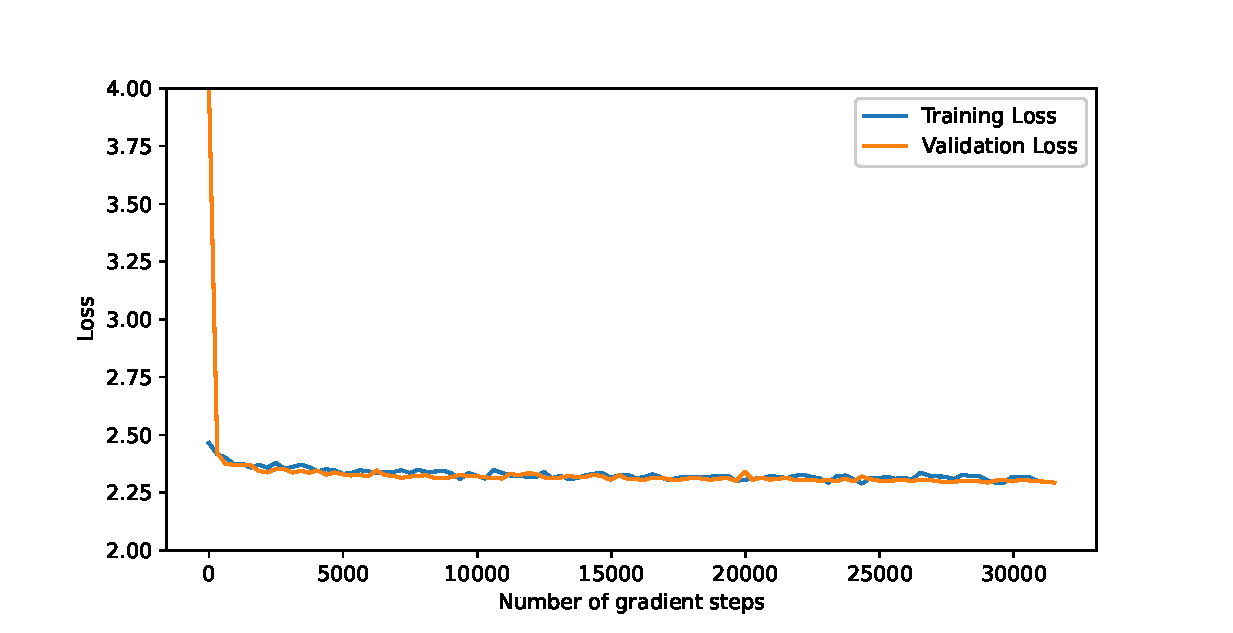
\includegraphics[width=\textwidth]{img/loss70.eps}
    \caption{Histogram of nodes for pseudo cost branching and MLP2.}
    \label{fig:node_histogram}
\end{figure}


\section{Linear Model Coefficients}\label{sec:coefficients}
...


\backmatter
\printbibliography[heading=bibintoc,title={References}]

\end{document}
